\chapter{پژوهش‌های پیشین}\label{chap2}
\minitoc

در این فصل برخی مدل‌های ارائه شده مرتبط با مسئله گپ‌زن دانش  ارائه و بررسی خواهند شد. در انتها نیز برخی دادگان جمع‌آوری شده در طی سالیان اخیر که می‌توانند برای مساله گپ‌زن دانش مفید واقع شوند معرفی شده اند.

\section{مدل‌های گپ‌زن دانش بنیان}\label{intro}

\subsection{مدل پیشنهاد شده توسط وینیالز}

این مدل در سال ۲۰۱۵ و بر پایه معماری دنباله به دنباله با استفاده از شبکه LSTM 
دو لایه با اندازه 
\trans{Hidden State }{حالت نهان}
۴۰۹۶
ارائه شد
\cite{A_Neural_Conversational_Model}.
این مدل در واقع فاقد منبع دانش خارجی است و صرفا از شبکه آموزش دیده شده روی دادگان آموزشی تشکیل شده است. اما اهمیت ذکر این مدل در اینجا، به دلیل نشان دادن این حقیقت است که حتی مدل‌های فاقد منبع دانش نیز  علاوه بر تقلید 
\trans{دستور زبان}{grammar}
 مکالمه انسانی، قادرند تا مقداری از حقایق جهان را در شبکه خود ذخیره کنند.
 برای مثال،‌ نمونه‌ای از گفتگوی چالشی دانش‌محور عامل انسانی با این مدل در شکل
 \ref{fig:chap2:Vinyals1}
 آورده شده است.

\begin{figure}[h]
	\centering
	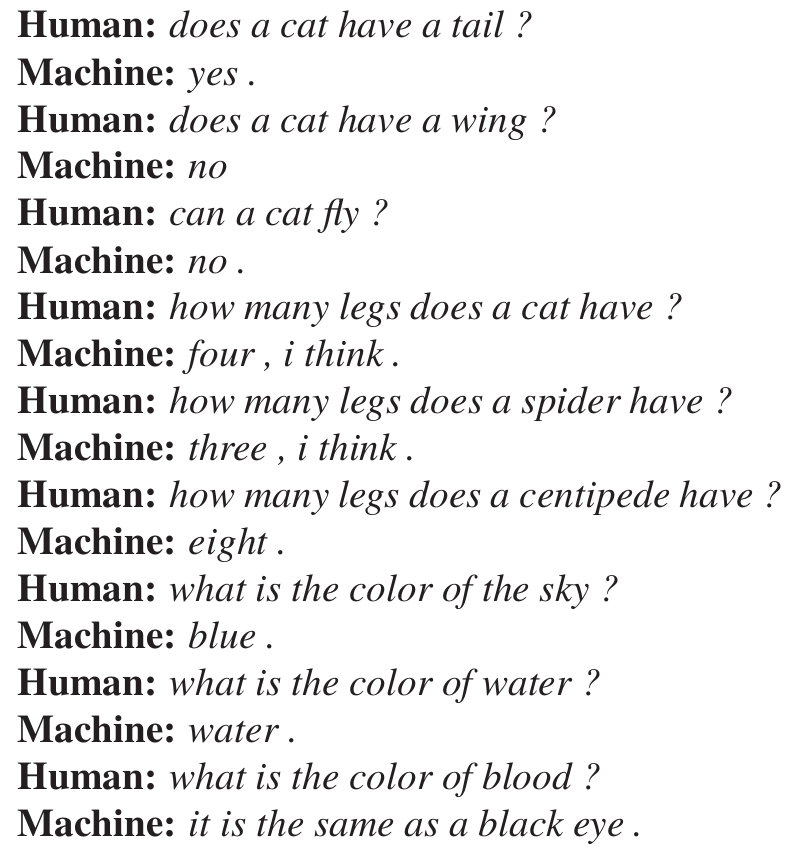
\includegraphics[width=0.75\textwidth]{images/chap2/Vinyals1.png}
	\caption{
		نمونه‌‌ای از گفتگوی چالشی دانش‌محور عامل انسانی با مدل وینیالز
		\cite{A_Neural_Conversational_Model} 
	}
	\label{fig:chap2:Vinyals1}
\end{figure}

همانطور که در شکل
\ref{fig:chap2:Vinyals1}
مشاهده‌ می‌شود مدل در پاسخ به سوالاتی مانند تعدادی پا‌های گربه و یا رنگ آسمان توانسته‌ است به خوبی پاسخ درست را خروجی دهد، حال آن که در موارد دیگری نظیری رنگ آب و یا تعداد پاهای عنکبوت نتوانسته‌است به موفقیت دست پیدا کند.

مدل وینیالز را می‌توان یکی از اولین تلاش‌های موثر در دستیابی به گپ‌زن دامنه باز دانست. این مدل سعی کرد تا با آموزش بر روی دادگان عظیم 
\lr{OpenSubtitle}
به این مهم دست یابد و توانایی این مدل در برخی استنتاج‌‌ها و پاسخگویی به سوالات چالشی دانش‌محور را نیز می‌توان به نوعی از تاثیرات حجم عظیم دادگان‌ آموزشی آن دانست.
\cite{Tiedemann2009NewsFO}
 پژوهش وینیالز علاوه بر موارد فنی مطرح شده، در زمینه آزمایش و ارزیابی مدل خود از آزمایشات جالب توجه و چالش بر‌انگیز  انجام مکالمات چالش برانگیز 
(نظیر آن‌چه که در شکل 
\ref{fig:chap2:Vinyals1}
به نمایش درآمد
)
استفاده کرد که می‌تواند نمونه‌ای‌ مناسب برای ارزیابی مدل‌های بعد از خود باشد. 

\subsection{مدل پیشنهاد شده توسط قزوینی نژاد}
این مدل را می‌توان به نوعی نخستین سامانه گپ‌زن تماما داده محوری دانست که به طور موثر از دانش بیرونی خود استفاده می‌کند
\cite{a_knowledge_grounded}.
انگیزه اصلی این مدل، این بوده است که از آنجایی که بخش عمده‌ای از دانش دنیا در دادگان آموزشی ارائه شده برای مسئله مکالمه حاضر نیستند، در نتیجه سامانه‌های مکالمه حاصل از آموزش روی این دادگان نیز نمی‌توانند عملکرد دانش‌مداری از خود ارائه دهند. از طرفی حتی اگر تمامی دانش دنیای بیرونی را بتوان در یک دادگان آموزشی گنجاند، این دادگان قطعا به حدی غیرقابل تصور بزرگ خواهد بود و قادر به آموزش مدل خود روی آن نیستیم
\cite{a_knowledge_grounded}.
در نتیجه برای حل مشکل دانش بنیان‌کردن سامانه‌ گپ‌زن این مقاله روشی را پیشنهاد داده است که در آن سعی کرده است از تکرار دانش در دادگان آموزشی پرهیز کند و از طرفی بتواند مدل مکالمه پایه را به گونه‌ای تعمیم دهد که قابلیت نمایش دانش رانیز داشته باشد. برای نیل به این هدف، این پژوهش سعی کرده است تا از حقایق موجود در پست‌های شبکه‌های اجتماعی نظیر توییتر و 
\lr{Four-Square} 
استفاده کند و به کمک آن‌ها پاسخ‌های با ارزش اطلاعاتی تولید کند.

به منظور آموزش این مدل گپ‌زن سه مجموعه دادگان جمع‌آوری شده است. دسته اول شامل ۱.۱ میلیون نظرات افراد در شبکه اجتماعی 
\lr{four square}
است که راجع به رستوران‌های آمریکا و کانادا اظهار شده است. این مجموعه جملات در واقع نقش حقایق جهان بیرونی را برای این مدل دارند. دسته دوم ۲۳ میلیون سه‌تایی‌های گفت و گو شده در
توییتر
هستند. این دسته دوم، در واقع نشان ستون فقرات مدل را دارند و برای این فراهم شده اند تا مدل بتواند نحوه کلی چگونگی مکالمه کردن را بیاموزد.
دسته سوم اما حدود ۱ میلیون زوج متشکل از یک توییت و پاسخ به آن هستند که  در مورد یکی از موجودیت‌های مطرح‌شده در مجموعه حقایق مدل (دسته اول دادگان) هستند.

در این مدل ابتدا تمرکز گفتگو تعیین می‌شود. این فرآیند تعیین تمرکز در حالات ساده و ابتدایی می‌تواند به صورت استخراج کلیدواژه‌های خاصی مثل نام شهر‌ها، شرکت‌ها و یا کالا‌ها از گفتگو و یا در حالت پیچیده‌تر به صورت تشخیص موجودیت‌های اسمی
گفتگو، صورت گیرد.
در مرحله بعد جملات مرتبط با تمرکز تعیین‌شده در پایگاه دانش که متشکل از جملات پست‌های کاربران در شبکه‌های اجتماعی توییتر
و
\lr{Four Square}
است مورد جستجو واقع شده و جملات مربوط از پایگاه دانش استخراج و به عنوان مجموعه حقایق ذخیره می‌شوند.
در ادامه تاریخچه گفتگو توسط یک رمزگذار که از نوع شبکه بازگشتی است به یک بردار با طول ثابت تصویر می‌شود. در ادامه برای شیوه و چگونگی رمزکردن حقایق و دخیل کردن آن‌ها، این مقاله از ایده 
\trans{شبکه‌های حافظه‌ای}{memory networks}
استفاده کرده است
\cite{weston2014memory}
. اگر
$u \in R^d$
را برداری 
حاصل از اعمال رمزنگار بازگشتی بر روی تاریخچه گفتگو فرض کنیم آنگاه روابط نظری مورد استفاده مدل برای دخیل کردن حقایق به شرح زیر هستند:

\begin{equation}\begin{split}
m_i &= Ar_i , A \in R^{d \times v} \\
c_i &= Cr_i , A \in R^{d \times v} \\
p_i &= softmax(u^T m_i) \\ 
o_i &= \sum_{i=1}^{k} p_i c_i \\
\hat{u} &= u + o
\end{split}\end{equation}

لازم به ذکر است که در عبارات فوق،
$r_i$
بردار
\trans{کیسه کلمات}{Bag of Words}
 حقیقت
$i$
ام است.
در صورتی که بخواهیم عبارت فوق را تفسیر کنیم، می‌توانیم این گونه بنگریم که بردار
$u$
در نقش یک بردار پرس و جو در یک مکانیزم شبیه به توجه، بر روی بردارهای 
$m$
مورد جستجو قرار می‌گیرد و در نهایت خروجی رمزگذار حقیقت، ترکیبی خطی (که ضریب هر جمله متناسب با میزان شباهت آن با بردار خلاصه تاریخچه گفتگو است)
از بردار‌های
$c$
متعلق به حقایق مختلف است.
سپس این بردار خروجی
$o$
با بردار خلاصه تاریخچه گفتگو جمع می‌شود و به عنوان حالت نهان اولیه به
رمزگشای پاسخ داده می‌شود که وظیفه آن تولید پاسخ برای نوبت بعدی گفتگو است. نمایی از معماری مدل ارائه شده توسط قزوینی‌نژاد در شکل
\ref{fig:chap2:qazvini-arch}
آمده است.

 \begin{figure}[H]
	\centering
	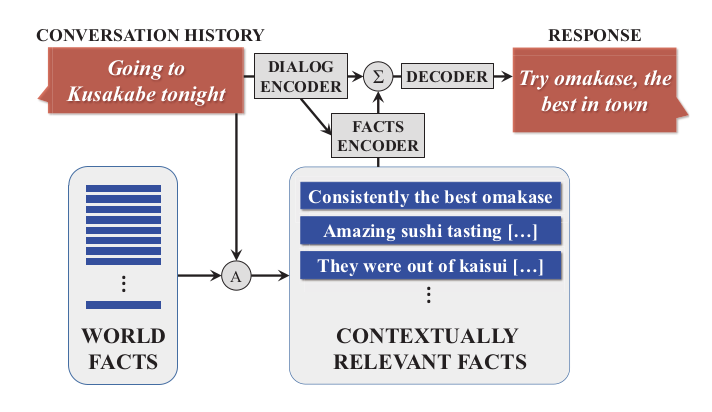
\includegraphics[width=0.75\textwidth]{images/chap2/qazvini-arch.png}
	\caption{نمایشی از معماری مدل مکالمه ارائه شده توسط قزوینی‌نژاد
		\cite{a_knowledge_grounded}}	
	\label{fig:chap2:qazvini-arch}
\end{figure}

ابتکار قابل ذکر این مقاله اما در چگونگی آموزش مدل است. به این صورت که با توجه به سه‌تایی موجود تاریخچه گفتگو، حقایق مرتبط با هر تاریخچه و پاسخ مطلوب تعدادی وظیفه منحصر به فرد تعریف شده‌اند. سپس مجموعه‌ای از ترکیب این وظایف با یکدیگر مشخص شده و مدل هر بار بر اجتماعی از این وظایف به صورت 
\trans{یادگیری چندوظیفه‌ای}{Multitask Learning}
آموزش می‌بیند. در نهایت نشان داده می‌شود که ترکیب این وظایف چگونه باعث بهبود عملکرد مدل می‌شود
\cite{a_knowledge_grounded}
.
در آخر، این پژوهش برای ارزیابی مدل پیشنهادی خود از دو دسته ارزیابی‌های
\trans{ذهنی}{subjective}
و
\trans{عینی}{objective}
استفاده می‌کند.
برای ارزیابی عینی از معیار‌های
\lr{BLEU}
و
\lr{Perplexity} 
بر روی پاسخ‌های تولیدشده استفاده می‌شود
\cite{papineni-etal-2002-bleu}
. برای ارزیابی ذهنی نیز، این پژوهش از نظرسنجی انسانی بر روی دو ملاک میزان مناسب بودن پاسخ تولیدشده و میزان آموزنده و با اطلاعات‌بودن پاسخ بهره برده است.


\subsection{مدل جادوگر ویکی‌پدیا} 

یکی از چالش‌های بزرگ بر سر راه گپ‌زن‌های دانش بنیان، عدم وجود دادگان و 
\trans{سنجه}{benchmark}
برای این وظیفه است. 
دینان در این پژوهش
در ابتدا به وسیله تعریف یک سناریو مشخص و 
\trans{جمع بسپاری}{crowdsourcing}
دادگانی را برای مسئله دانش بنیان کردن گپ‌زن‌ها جمع آوری نموده است و سپس با بهره‌گیری از ترنسفورمر‌ها 
معماری را ارائه کرده است که قابلیت بازیابی دانش و تولید پاسخ مشروط به دانش را داراست
\cite{wizard}. 

سناریویی که برای جمع آوری دادگان در نظر گرفته شده است به این شرح است که ابتدا موضوعی به صورت تصادفی تعیین می‌شود و قرار است که در ادامه دو نفر درباره این موضوع با یکدیگر گفتگو کنند، به علاوه ممکن است این موضوع در طی گفتگو گسترده‌تر شود یا این که به موضوعات مرتبطش متمرکز شده و تغییر پیدا کند. این دو نفر دو نقش متفاوت را در این سناریو بازی می‌کنند به این معنی که یک نفر نقش شاگرد کنجکاو را دارد و بیشتر در پی کشف اطلاعات در مورد موضوع مورد گفتگو و عمیق کردن بحث در مورد آن است و طرف مقابل در نقش استاد است که در مورد موضوع مورد گفتگو اطلاعات کاملی را دارد و هدفش انتقال اطلاعات در مورد موضوع به طرف مقابل است
\cite{wizard}.

روند یک گپ‌ میان استاد و شاگرد به این صورت است که ابتدا یکی از طرفین به تصادف انتخاب شده و موضوعی را انتخاب می‌کنند و راجع به آن سخن می‌گوید. سپس هر موقع که شاگرد پیامی را به استاد بفرستد، به استاد لیستی از دانش‌های مربوط به گفتگوی فعلی نمایش‌ داده می‌شود؛ استاد یکی از جملات را انتخاب می‌کند و با توجه به آن پاسخی به شاگرد می‌دهد(استاد همچنین می‌تواند هیچ جمله‌ای را انتخاب نکند).
این مکالمه در نهایت پس از حداقل چند نوبت رد و بدل شدن پیام به صورت تصادفی پایان می‌پذیرد.
حال پس از جمع‌ آوری دادگان هدف جایگزینی نقش استاد با یک سامانه مکالمه‌گر است
\cite{wizard}
.

به این منظور این مقاله معماری را ارائه کرده است که از سه بخش تشکیل شده است. بخش اول مسئول بازیابی دانش از صفحات ویکی‌پدیا، بخش دوم مسئول مطالعه و توجه به مجموعه دانش‌های بازیابی شده و در نهایت بخش سوم نیز مسئول تولید کردن پاسخ نوبت بعدی گفتگو هستند.

برای بخش اول از یک 
\trans{پیمانه}{Module}
\trans{بازیابی اطلاعات}{Information Retreival}
 ارائه شده در 
مدل ارائه شده توسط دنگی چن در ۲۰۱۷
استفاده شده است که وظیفه آن  پیدا کردن صفحات مرتبط با گفتگو از ویکی‌پدیا است
\cite{drqa_paper}
. پس از پیدا شدن صفحات مرتبط پاراگراف اول آن صفحات (که معمولا خلاصه‌ای از آن صفحه هستند) برداشته می‌شوند و به جملاتشان می‌‌شکنند. سپس به ابتدای هر جمله عنوان صفحه آن اضافه شده و جملات برای استفاده در مرحله بعدی ذخیره می‌شوند. 

هدف بخش دوم از معماری یعنی قسمت توجه به دانش، این است که با توجه به تاریخچه گفتگو و جملات استخراج شده از بخش اول، جمله اصلی مرتبط با گفتگو را حدس زده و آن را تعیین کند. این بخش از معماری از یک ترنسفورمر بهره برده است به این شکل که تاریخچه گفتگو و هر یک از جملات استخراج شده در بخش اول با یک ترنسفومر مشابه ولی به صورت جدا و مستقل از هم به یک بردار با طول ثابت رمز می‌شوند. سپس استفاده از ضرب داخلی میزان مشابهت بردار رمز  گفتگو با بردارهای رمز جملات دانش مشخص می‌شود. سپس این میزان مشابهت‌ها از یک لایه 
\lr{softmax}
عبور کرده و با توجه به خطای 
\lr{cross-entropy}
و همچنین جمله‌ای که در دادگان آموزشی به عنوان جمله مرتبط در هنگام تولید پاسخ توسط استاد انتخاب شده است، میزان خطا و تابع هزینه آن مشخص می‌شود.

 در این قسمت مقاله دو رویکرد متفاوت را برای پیاده‌سازی بخش دوم و سوم اتخاذ کرده است. در رویکرد اول که آموزش انتها به انتها است، بردار‌های رمز  تاریخچه گفتگو و جمله دانشی که بیشترین مشابهت با آن را دارد با یکدیگر الحاق می‌شوند و در بخش سوم معماری به یک ترنسفورمر رمزگشا داده می‌شوند و کل بخش دوم و سوم با یکدیگر آموزش می‌بینند.
تابع هزینه‌ای هم که برای آموزش کل این دو بخش مورد استفاده قرار می‌گیرد عبارت زیر است.


\begin{equation}\begin{split}
\mathcal{L} = (1- \lambda ) \mathcal{L}_{NIL} + (\lambda) \mathcal{L}_{knowledge}
\end{split}\end{equation}

که در عبارت بالا
$\mathcal{L}_{NIL}$
میزان خطای رمزگشا به هنگام تولید پاسخ
،
$\mathcal{L}_{knowledge}$
میزان خطای بخش توجه به دانش برای انتخاب جمله صحیح مرتبط
و
$\lambda$
نیز یک ضریب تنظیم‌گر بین خطای انتخاب دانش و تولید پاسخ درست هستند.

اما در رویکرد دوم که آموزش دو مرحله‌ای بخش دوم و سوم است، هر کدام از بخش ‌های دوم و سوم جداگانه آموزش می‌بینند. در این رویکرد پس از انتخاب جمله دانش مرتبط، این جمله و تاریخچه گپ دوباره و با هم با یک ترنسفورمر رمز می‌شوند و سپس وارد ترنسفورمر رمزگشا می‌شوند. از آن جایی که رخدادن خطا در بخش دوم می‌تواند موجب انتشار خطایی قابل توجه برای بخش سوم شود و به نوعی حتی این نوع آموزش دادن دو مرحله‌ای موجب
\trans{بیش‌برازش}{Overfitting}
 بخش سوم روی بخش دوم شود، این مقاله ایده‌ی 
 \trans{حذف تصادفی}{Dropout}
 روی دانش را مطرح کرده است، که در آن به مانند ایده حذف تصادفی
،بخش سوم در مواقعی بایستی بدون دانستن جمله مرتبط   پاسخ صحیح را بتواند تولید کند
\cite{wizard}.

  جهت فهم و درک بهتر نمایی از معماری این دو رویکرد در شکل
\ref{fig:chap2:wizard-arch}
آمده است.

 \begin{figure}[H]
	\centering
	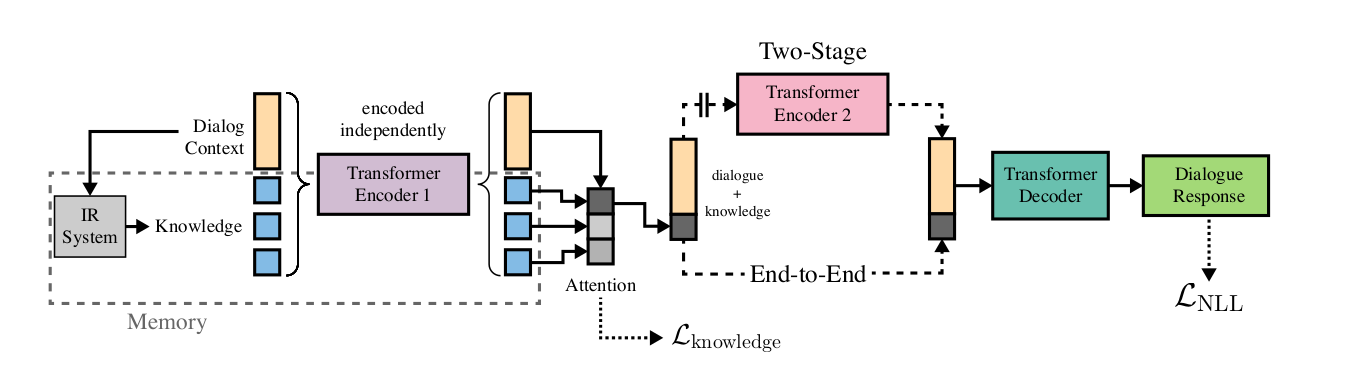
\includegraphics[width=1\textwidth]{images/chap2/wizard_arch.png}
	\caption{نمایشی از معماری مدل مکالمه جادوگر ویکی‌پدیا
		\cite{wizard}}	
	\label{fig:chap2:wizard-arch}
\end{figure}


\subsection{پیش‌نیازها}
\iffalse
	قرارداد می‌کنیم توزیع $P$ مربوط به توزیع داده واقعی باشد و در مقابل آن به دنبال یافتن توزیع $Q$ هستیم که تا حد ممکن نزدیک به $P$ باشد.
	از آنجا که در طول متن گزارش، فاصله‌های گوناگونی مورد استفاده قرار گرفته است، در ابتدا آن‌ها تعریف می‌کنیم. در تمامی تعاریف، P مربوط به توزیع اصلی و Q مربوط به توزیعی است که یاد گرفته می‌شود.
\fi
\subsubsection{معیارهای فاصله بین دو توزیع} \label{chap2:divs}
پیش از توضیح روش‌های مختلف ابتدا  لازم به ذکر است تمامی این فواصل بین دو توزیع $p$ و $q$ تعریف شده‌اند.
\\
\bff{فاصله \lr{KL}} \cite{bishop}:
\begin{gather} \label{eq: kl}
	KL (p ~ || ~ q)   = \sum_x p(x) \log \frac{p(x)}{q(x)}
\end{gather}
اگر $p$ توزیع داده باشد و به دنبال یادگیری $q$ باشیم، کمینه کردن فاصله فوق همان روش \maxlikelihood{} خواهد بود.
\\
\bff{فاصله \lr{KL} برعکس}:
\begin{gather} \label{eq: rkl}
	KL (q ~ || ~ p)   = \sum_x q(x) \log \frac{q(x)}{p(x)}
\end{gather}
مجددا اگر $p$ توزیع داده باشد، از آنجا که دسترسی به آن وجود ندارد، فاصله فوق به صورت مستقیم قابل بهینه‌سازی نیست.
\\
\bff{فاصله \lr{Jensen Shannon}}:
\begin{gather} \label{eq: js}
	JS (p ~ || ~ q)   = KL(p ~ || ~ \frac{p + q}{2}) + KL(q ~ || ~ \frac{p + q}{2})
\end{gather}
این فاصله بر خلاف دو فاصله قبلی، نسبت به جابه‌جایی $p$ و $q$ حساس نبوده و \gan{} در تئوری، این فاصله را کمینه می‌کنند \cite{gan}.
\\
\bff{فاصله
	\trans{واسرشتاین}{Wasserstein}}:
فرض کنید می‌خواهید تعداد مشخصی جعبه که به ترتیب خاصی بر روی یکدیگر و کنار هم قرار گرفته‌اند را به مکانی دیگر منتقل کنید. برای مثال طبق شکل \ref{fig:chap2:wasser1} میخواهید مربع‌های سمت چپ را به مکان‌های با نقطه‌چین مشخص شده منتقل کنید. به صورت‌های مختلفی می‌توان این کار را انجام داد. دو نمونه از این جابه‌جایی در شکل \ref{fig:chap2:wasser2} آمده است.
\begin{figure}[h]
	\centering
	\begin{subfigure}[t]{.7\textwidth}
		\centering
		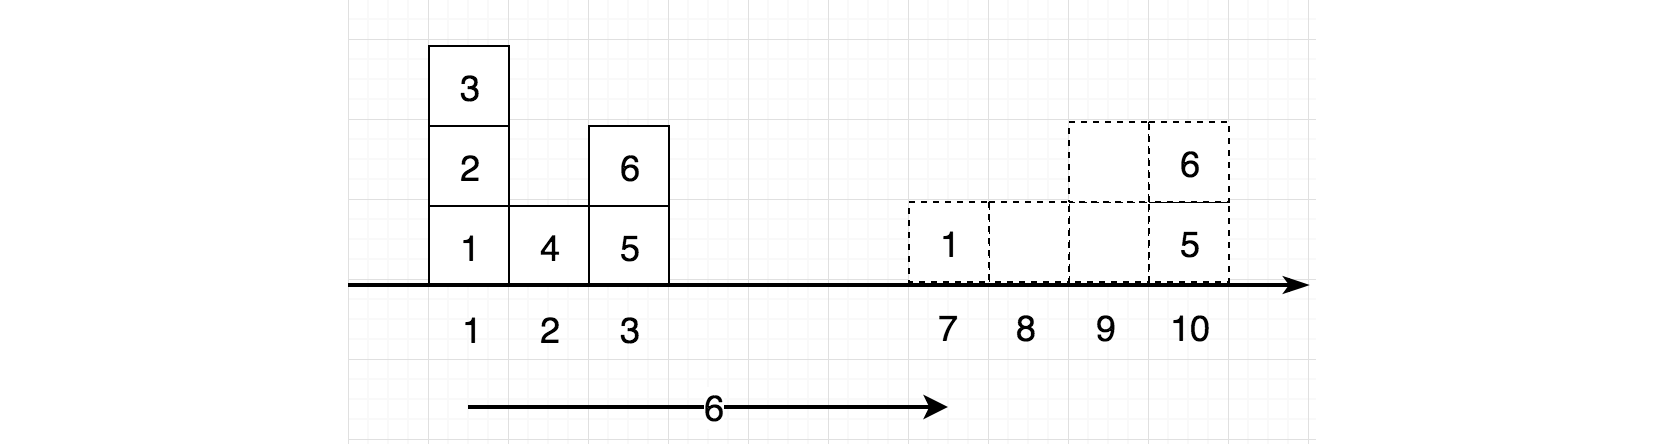
\includegraphics[width=1.\textwidth]{images/wasser2.png}
		\caption{}
		\label{fig:chap2:wasser1}
	\end{subfigure}

	\begin{subfigure}[t]{.6\textwidth}
		\centering
		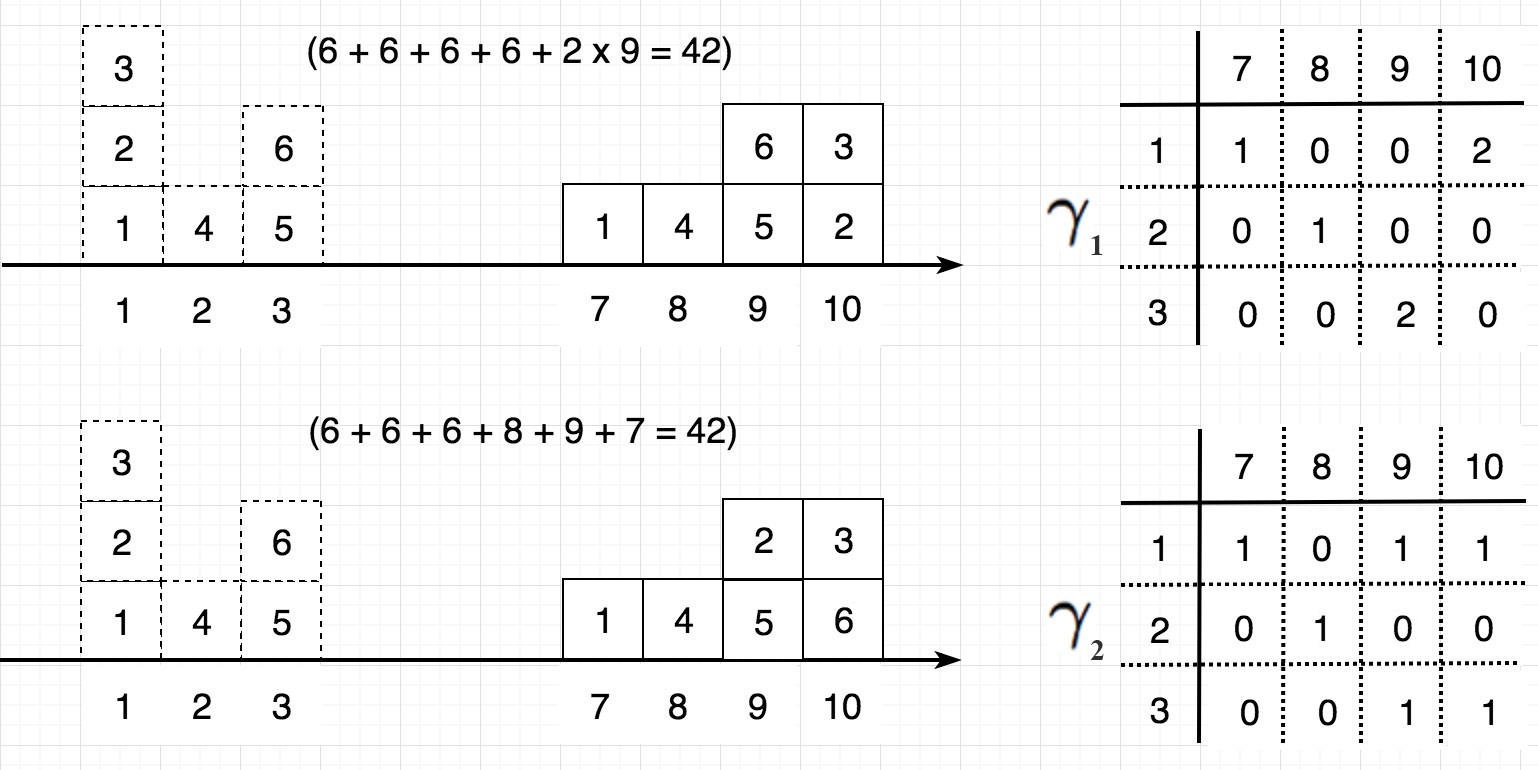
\includegraphics[width=1.\textwidth]{images/wasser1.jpeg}
		\caption{}
		\label{fig:chap2:wasser2}
	\end{subfigure}
\caption{
    مثالی از دو توزیع \subref{fig:chap2:wasser1} و 
    \transportplan{} 
    بین دو توزیع \subref{fig:chap2:wasser2}}
\end{figure}
اگر $\gamma$ را یک
\trans{طرح جابه‌جایی}{Transport Plan}
بنامیم که به صورت جدولی که سطرها مکان اولیه جعبه‌ها و ستون‌ها مکان ثانویه جعبه‌ها نشان داده و هر خانه آن نشان دهنده تعداد جعبه‌ی جابه‌جا شده از نقطه اولیه به ثانویه است، جمع عناصر این جدول برابر هزینه جابه‌جایی کلیه جعبه‌ها خواهد بود. از آنجا که \transportplan{} واحدی به این منظور وجود ندارد، \transportplan{} با کمترین هزینه جابه‌جایی برابر فاصله \wasser{} بین حالت اولیه و ثانویه جعبه‌ها است.
\\
به منظور تعریف دقیق‌تر، اگر دو توزیع به نام‌های $q$ و $p$ داشته باشیم، فاصله \wasser{} برابر کمترین هزینه جابه‌جایی برای جابه‌جایی جرم توزیع $p$ به $q$ خواهد بود.
اگر مجموعه تمام توزیع‌های توام $\gamma(x,y)$ که توزیع‌های \marginal{} آن به ترتیب برابر $p$ و $q$ باشد را با $\Pi(p,q)$ نشان دهیم، فاصله \wasser{} به صورت زیر تعریف می‌شود:
\begin{align}
	W_c(p,q) = \inf_{\gamma(x,y) \in \Pi(p,q)} \expected_{(x,y) \sim \gamma(x,y)} [ c(x,y) ]
\end{align}
و $c$ یک متر تعریف شده بر روی این فضا و اندازه‌گیرنده هزینه جابه‌جایی بین دو نقطه است. به طور شهودی توزیع توام $\gamma$ نشان دهنده جرم جابه‌جا شده از نقطه $x$ به نقطه $y$ است به طوری که تمام جرم از توزیع $p$ به توزیع $q$ منتقل شود. در حالتی که $c = ||x-y||$ باشد، به فاصله فوق فاصله \earthmover{} نیز گفته می‌شود.
\\
از آنجا که کمینه کردن فاصله فوق معمولا سخت است، طبق فرم دوگان \lr{Kantorovich-Rubinstein } فاصله \earthmover{} برابر است با \cite{wgan}:
\begin{align}
	W(p, q) = \sup_{||f||_L \leq 1} \expected_{x \sim p(x)}[f(x)] - \expected_{x \sim q(x)}[f(x)]
\end{align}
که سوپریمم بر روی تمام توابع $f$ با ضریب \lipschitz{} حداکثر یک گرفته شده است. شرط \lipschitz[K-]{} که به صورت
$|f(x) - f(y)| \leq K |x - y|$
به ازای تمام $x$ و $y$ ها تعریف می‌شود به طور شهودی به معنای توابعی است که چندان تغییرات شدیدی ندارند.
\\
از این فاصله به عنوان تابع هدف جدید در \gan{} استفاده شده که به \wgan{} معروف است. نکته قابل توجه این است که چون تابع $f$ فوق چندان انحنای شدیدی ندارد، حتی در صورت دور بودن توزیع داده واقعی و مصنوعی، همچنان تابع $f$ به صورت محلی احتمالا خطی بوده و گرادیان از \discriminator{} به \generator{} بر خواهد گشت \cite{wgan}. نمایی از این تفاوت گرادیان دو نوع  \gan{} در شکل \ref{fig:chap2:wgan1} مشخص است.
\begin{figure}[h]
	\centering
	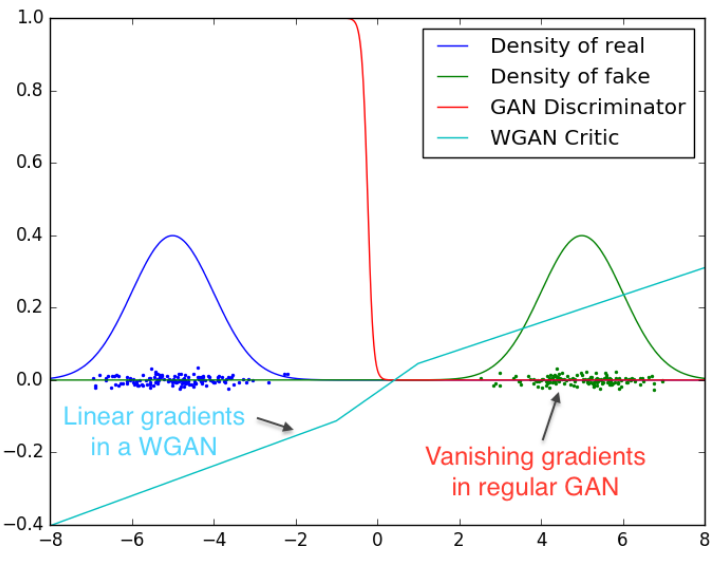
\includegraphics[width=0.5\textwidth]{images/wgan1.png}
	\caption{
        تفاوت خروجی \discriminator{} در \gan{} عادی و \wgan{} (\lr{WGAN})
        \cite{wgan}
    }
	\label{fig:chap2:wgan1}
\end{figure}
\\
\bff{فاصله 
    \trans{بیشینه اختلاف میانگین}{Maximum Mean Disrepancy (\mmd{})} (\mmd{})}:
برای تابع کرنل مثبت معین 
\trans{‎با قابلیت بازتولید}{Reproducing}
$k: ‎\mathcal{Z} ‎‎\times \mathcal{Z} ‎\rightarrow ‎\mathbb{R}‎‎$
رابطه ‎\mmd{} به شکل زیر تعریف می‌شود:
\begin{gather}
	\mathsf{MMD}_k(p, q) = {\vert \vert \int_\mathcal{X} k(x, .) dp(x) - \int_\mathcal{X} k(x, .) dq(x) \vert \vert}_{\mathcal{H}_k}
\end{gather}
به طوری که $‎\mathcal{H}‎_k$، یک 
\trans{کرنل با قابلیت بازتولید در فضای هیلبرت}{Reproducing ‎ Kernel ‎ Hilbert ‎ Space (RKHS)}،
برای توابع از $‎\mathcal{X}‎$ به اعداد حقیقی است. اگر تابع $k$ ویژگی‌های مشخصی را داشته باشد، ‎\mmd{}‎ را به یک متر تبدیل کرده و این امکان را فراهم می‌کند تا از این متر به عنوان تابع هزینه برای کمینه کردن فاصله دو توزیع $p$  و $q$  بهره برده شود. از آنجا که رابطه بالا به طور مستقیم قابل محاسبه و بهینه‌سازی نیست، از تخمین‌گر 
\trans{نااریب}{Unbiased}
 زیر استفاده می‌گردد. اگر $n$ نمونه از دو توزیع $p$ و $q$ داشته و به ترتیب با $x_i$ و $‎\tilde{x}_i$ نشان داده شوند،‌خواهیم داشت:
\begin{align}
	\mathsf{MMD}_k(x_{1,2,...,n};\tilde{x}_{1,2,...,n}) = & \frac{1}{n(n-1)} \sum_{l \neq j} k(x_l, x_j) +
	\frac{1}{n(n-1)} \sum_{l \neq j} k(\tilde{x}_l, \tilde{x}_j)                            \nonumber         \\
	                                                      & - \frac{1}{n ^ 2} \sum_{l, j} k(x_l, \tilde{x}_j)
\end{align}
فاصله فوق با کرنل
$k(x, y) = \frac{C}{C + ||x - y||^2_2}$
برای فاصله بین دو توزیع گاوسی کاربرد دارد و به خوبی عمل می‌کند \cite{wae}.

\section{مدل‌های زبانی بدون فضای نهان}
\subsection{مدل زبانی پایه (\teacherforcing{})}
مدل \teacherforcing{} شاید ساده‌ترین دسته از مدل‌های تولید متن با استفاده از شبکه‌های عصبی باشد. آموزش این مدل‌ها مبتنی بر بیشینه کردن \likelihood{} داده آموزش در مدل است \cite{teacher_force} اگر پارامترهای مدل را با $‎\theta$ نشان دهیم، تابع هزینه این مدل به صورت زیر است:
\begin{equation}\begin{split}
		L_{MLE} = -\expected_{\bff{x} \sim p_{data}(\bff{X})} [\log p_\theta (\bff{x})] = -\expected_{\bff{x} \sim p_{data}(\bff{X})} [\log p_\theta (\bff{x}_1) + \sum_{t=2}^{T}  \log p_\theta (\bff{x}_t|\bff{x}_1, ..., \bff{x}_{t-1})].
	\end{split}\end{equation}

\begin{figure}[H]
	\centering
	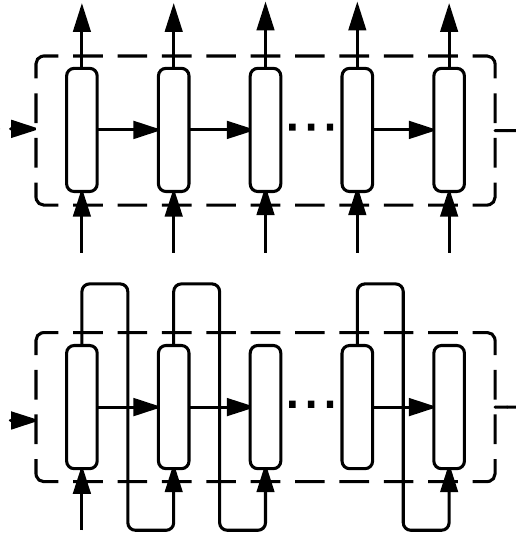
\includegraphics[width=0.25\textwidth]{images/teach-prof.png}
	\caption{
		تفاوت بین آموزش و آزمون مد‌ل جبر معلم. شکل بالا مربوط به زمان آموزش و شکل پایین مربوط به زمان آزمون است. \cite{prof_force}.}
	\label{fig:chap2:expbias}
\end{figure}

به عبارت دیگر، در هر زمان درست‌نمایی هر کلمه را با داشتن کلمات قبلی بیشینه می‌کنیم. \\
همان‌طور که از روابط تابع هزینه مشخص است، آموزش این دسته از مدل‌ها ساده بوده اما دچار پدیده‌ای به نام 
\trans{اریبی مواجهه}{Exposure bias}
 هستند \cite{ prof_force, s_sampling}. این مشکل ناشی از تفاوت رفتار با مدل حین آموزش و حین آزمون است. همان طور که در شکل \ref{fig:chap2:expbias} مشخص است، حین آموزش، در هر زمان، کلمات کاملا درست تحویل مدل شده، در حالی که در زمان آزمون ورودی شبکه در هر زمان، با استفاده از نمونه‌گیری از خود مدل در زمان قبل ساخته می‌شود. از آنجا که مدل مفهوم کاملا درستی را نیاموخته است، کلمه‌ی تولید شده برای ورود به زمان بعد، کلمه کاملا صحیحی نبوده و چنین رفتاری باعث می‌شود تا مدل، ورودی‌ای را دریافت کند که دارای مقداری خطا بوده که در زمان آموزش مانند آن را ندیده است (در زمان آموزش کلمات کاملا صحیح ورودی شبکه بوده‌اند)؛ این رفتار در طول تولید هر کلمه از یک جمله با هم تجمیع شده و در نهایت منجر به تولید جمله‌ای نه چندان صحیح خواهد شد.\\
به منظور رفع این مشکل، روش‌های متفاوتی ارائه شد \cite{prof_force, s_sampling, seqgan} که در بخش \ref{chap2:seqgan} به عنوان یکی از راه‌حل‌ها به آن پرداخته خواهد شد.
از دیگر مشکلات این روش باید به تفاوت تابع هزینه و معیار ارزیابی اشاره کرد؛ به عبارت دیگر اگر معیار ارزیابی، معیاری مانند \lr{BLEU} باشد، هدف ارزیابی کسب امتیاز بالاتر \lr{BLEU} است و نه افزایش درست‌نمایی داده آموزش و لزوما افزایش درست‌نمایی به افزایش ‌\lr{BLEU} منجر نمی‌شود.
\subsection{مدل زبانی با استفاده از \gan{}}
شاید \gan{} یکی از مطرح‌ترین و موفق‌ترین مدل‌های مولد حال حاضر باشند. این شبکه‌ها که مجددا ابتدا در حوزه تصویر معرفی شدند، از دو بخش کلی تشکیل شده اند \cite{gan}؛ بخش 
\generator{}
  و بخش 
\discriminator{}.
  همان‌طور که از نام‌گذاری آن‌ها مشخص است، مولد وظیفه تولید نمونه‌های مصنوعی و \discriminator{} وظیفه تشخیص نمونه مصنوعی از واقعی را دارد. نحوه آموزش آن‌ها به این صورت است که مولد سعی در تولید نمونه‌های شبیه به داده واقعی داشته و \discriminator{} در جهت مخالف سعی در شناسایی این نمونه‌ها دارد. در واقع نوعی 
\trans{بازی کمینه-بیشینه}{Min-max game}
بین مولد و \discriminator{} در جریان است. تابع هدف این مدل به شرح زیر است \cite{gan}:
\begin{equation} \label{eq:gan}
	\begin{split}
		V_{GAN} (G, D) = \expected_{\bff{x} \sim p_{data}(\bff{X})} [\log D(\bff{x})] + \expected_{\bff{z} \sim p(\bff{Z})} [\log (1 - D(G(\bff{z})))]
	\end{split}
\end{equation}
که  $p(\bff{z})$ توزیع پیشین تعریف شده بر روی نویز $\bff{z}$،
$G(\bff{z})$
تابع مولد (تبدیل کننده نویز $\bff{z}$ به نمونه $\bff{x}$)، $D(\bff{x})$ تابع \discriminator{} بوده و این رابطه برحسب $G$ کمینه و $D$ بیشینه می‌گردد.\\
اگر $q_G(\bff{x})$ نشان دهنده توزیع حاصل از اعمال تابع $G(\bff{z})$ به توزیع پیشین $p(\bff{z})$ باشد؛ نشان داده شده است که نقطه بیشینه کننده رابطه \ref{eq:gan} بر حسب $D$، به صورت زیر است \cite{gan}:
\begin{gather}
	D_G^*(\bff{x}) = \frac{p_{data}(\bff{x})}{p_{data}(\bff{x}) + q_G(\bff{x})}
\end{gather}
با فرض رسیدن به \discriminator{} بهینه، کمینه کردن $V(D^*_G,G)$ معادل کمینه کردن فاصله \lr{Jensen Shannon} بین $p_{data}(\bff{x})$ و $q_G(\bff{x})$ خواهد بود.

همان طور که اشاره شد \gan{}، ابتدا در حوزه تصویر معرفی شده و به دلیل عدم امکان عبور گرادیان که در ادامه شرح داده خواهد شد، چندان در حوزه متن موفق نبود. این مشکل از نحوه آموزش نشأت می‌گیرد. همان طور که در روابط تابع هزینه مشخص است، \discriminator{} باید به نمونه‌های تولید شده توسط مولد عددی نزدیک به صفر نسبت دهد. آنچه که باید در آموزش و الگوریتم 
\trans{گرادیان کاهشی تصادفی}{Stochastic gradient descent}
محاسبه شود، محاسبه مشتق تابع هزینه نسبت به پارامتر‌های شبکه مولد است؛ اما از آنجا که شبکه مولد مستقیما در تابع هزینه شرکت نکرده و نمونه‌های تولیدی آن شرکت می‌کنند و عملیات نمونه‌گیری در فضای گسسته عملیاتی مشتق‌ناپذیر است، بنابراین امکان گذر گرادیان از تابع هزینه (شبکه \discriminator{}) به شبکه مولد به سادگی وجود ندارد. در واقع شبیه چنین مشکلی در شبکه‌های \vae{} نیز وجود دارد اما با تکنیکی به نام
\trans{پارامتری‌سازی مجدد}{Reparameterization}
که منبع تزریق عامل تصادفی (نمونه‌گیری) را از مسیر انتقال گرادیان خارج می‌کند، حل شده است \cite{vae}.\\
به منظور حل این مشکل نیز رویکرد‌های متفاوتی ارائه شده است که به یکی و شاید معروف‌ترین از آن‌ها اشاره خواهد شد \cite{seqgan, gumbel}.\\
\subsubsection{\lr{SeqGAN}}  \label{chap2:seqgan}
در روش \lr{SeqGAN} راه حل ارائه شده برای مشکل گذر گرادیان الهام گرفته شده از حوزه 
\trans{یادگیری تقویتی}{Reinforcement Learning}
است \cite{seqgan}؛ در واقع همین مشکل به نوعی دیگر در حوزه یادگیری تقویتی مطرح است و با روشی به نام روش 
\trans{گرادیان سیاست}{Policy gradient}
 رفع شده است. ساختار یک مسئله حوزه یادگیری تقویتی شامل ۴ بخش است که با تعریف تمام بخش‌های آن، ‌می‌توان بخش آموزش مولد در \gan{} را به عنوان آموزش یک عامل با روش \reinforce{} دید. این بخش‌ها شامل موارد روبرو هستند: فضای حالت عامل ($S$)، فضای عمل عامل ($A$)، 
\trans{تابع گذار}{Transition function}
(\lr{$T(s,a)$})
و 
\trans{تابع پاداش}{Reward function}
(\lr{$R(s,a)$}).
\begin{equation}\begin{split}
		\nonumber
		T: S \times A \rightarrow S\\
		R: S \times A \rightarrow \mathbb{R}
	\end{split}\end{equation}
در اینجا حالت فعلی عامل، 
\trans{بازنمایی}{Representation}
کلمات تولید شده تا به حال است؛ عمل عامل،‌ کلمه انتخابی بعدی؛ حالت بعدی، تجمیع کلمات قبلی تولید شده و کلمه فعلی و در نهایت تابع پاداش، امتیاز میزان واقعی بودن جمله است که تمایز دهنده به جمله تولیدی نسبت می‌دهد. بدیهی است که تابع گذار تابعی 
\trans{قطعی}{Deterministic}
بوده و پاداش مورد نظر بعد از تولید کامل جمله به عامل داده می‌شود. در این حالت رابطه گرادیان تابع مولد به شکل زیر بدست خواهد آمد \cite{seqgan}.
\begin{equation} \label{eq:seqgan-grad}
	\begin{split}
		\nabla_G L_{GAN} (G, D) &= \nabla_G \expected_{\bff{x} \sim G(\bff{X})} [\log D(\bff{x})]= \expected_{\bff{x} \sim G(\bff{X})} [\log D(\bff{x}) \nabla_G \log G(\bff{x})].
	\end{split}
\end{equation}

\begin{figure}[t]
	\centering
	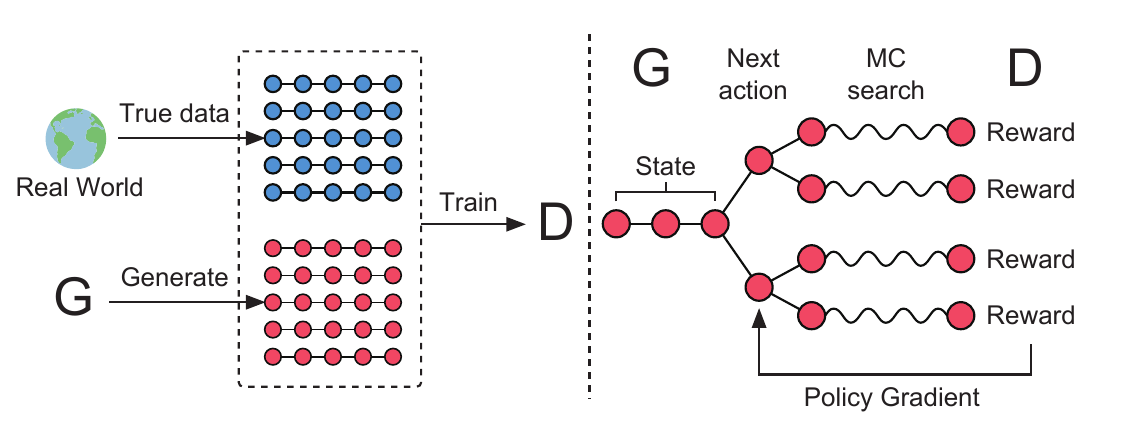
\includegraphics[width=0.5\textwidth]{images/seq-gan.png}
	\caption{
		نمایی نحوه آموزش مدل \lr{SeqGAN}
		\cite{seqgan}.}
	\label{fig:seq-gan}
\end{figure}

همان‌طور که در شکل \ref{fig:seq-gan} و رابطه \ref{eq:seqgan-grad} مشخص است، عامل طبق سیاستی که تا به حال بدست آورده است، تعدادی نمونه ایجاد نموده و به نسبت پاداش دریافتی به ازای هر نمونه، درست‌نمایی نمونه‌های مرتبط را افزایش خواهد داد.\\
نکته قابل توجهی که لازم است به آن اشاره شود، توانایی این روش در حل مشکل \expbias{} است. در واقع از یک سو در هر زمان کلمه بعدی توسط خود مدل تولید می‌شود و از سوی دیگر پاداشی که از \discriminator{} دریافت می‌کند، میزان  واقعی بودن کل جمله است؛ بنابراین اگر جمله تولید شده از نظر \discriminator{}، کیفیت لازم را نداشته باشد، \discriminator{} امتیاز کمتری به آن نسبت خواهد داد و گرادیان متناسب به مولد اعمال خواهد شد. با وجود آنکه این روش مشکل ذکر شده را حل می‌کند، اما فضایی که عامل باید در آن به دنبال یافتن پاداش بیشینه باشد نمایی بوده و همین امر آموزش این دسته از مدل‌ها را با چالش روبرو می‌کند. پیشنهاد ساده‌ای که برای این موضوع ارائه می‌شود استفاده از پیش آموزش به روش \teacherforcing{} است. در واقع ابتدا مدل به یک 
\trans{بهینه محلی}{Local optimum}
رسیده و در فضای نزدیک به آن احتمالا پاداش بیشتری نسبت به حالتی که مدل تصادفی باشد دریافت کرده و به اصلاح خود می‌پردازد.\\
این روش تنها مدل موجود با چنین رویکردی نبوده و روش‌هایی همچون \cite{pg_bleu} از دانش خبره مانند معیار \lr{BLEU} به عنوان پاداش بهره برده‌اند.
\section{مدل‌های زبانی با فضای نهان}
\subsection{خودکدنگار وَردِشی}
با معرفی \vae{}،
موج جدیدی در حوزه مدل‌های مولد به طور خاص مدل‌های مولد تصویر ایجاد شد.
\begin{figure}[H]
	\centering
	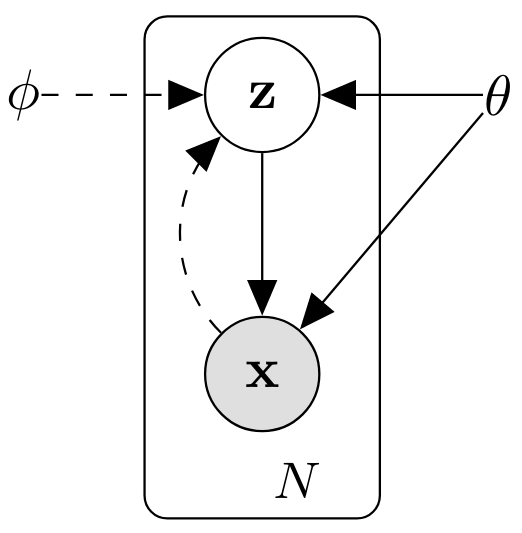
\includegraphics[width=0.25\textwidth]{images/vae-pgm.png}
	\caption
    [نمایی از مدل گرافی مورد استفاده در \vae{}.]
    {
		نمایی از مدل گرافی مورد استفاده در \vae{}. خطوط خطچین‌‌دار مربوط به تخمین توزیع پسین $p_\theta(\bff{z}|\bff{x})$ و خطوط بدون خطچین مربوط به مدل مولد
		$p_\theta(\bff{x}|\bff{z})$
		است.
		\cite{vae_text}.}
	\label{fig:vae-pgm}
\end{figure}
این ساختار به منظور یادگیری و 
\trans{استنتاج}{Inference}
مدل‌های با مدل گرافی نشان داده شده در شکل ‎\ref{fig:vae-pgm}‎ ارائه شده است. در واقع در این مدل، هر داده از یک 
\trans{متغیر نهان}{Latent Variable}
  تولید شده که \priordist{} مشخصی برای آن تعریف شده است و معمولا توزیع گاوسی نرمال است. از آنجا که محاسبه $\log p_\theta(\bff{x})$ و $\log p_\theta (z|x)$ نیازمند \inference ی 
\trans{سخت}{Intractable}
است، با بهره‌گیری از  توزیع وردشی $q_\phi(z|x)$، کران پایینی از \likelihood{} به نام \lr{ELBO} بیشینه می‌گردد.\\
از دیدگاهی دیگر، این مدل از دو بخش کلی تشکیل شده است؛ \encoder{} و \decoder{}. بخش \encoder{} وظیفه کد کردن داده ورودی در فضای نهان را داشته و در مقابل \decoder{} وظیفه برگرداندن فضای نهان به داده اصلی. تفاوت این مدل‌ها با \autoencoder{}ها در فرض و اعمال توزیع نرمال بر فضای نهان است؛ به همین دلیل امکان نمونه‌برداری از فضای نهان امکان‌پذیر خواهد بود. تابع هزینه در این ساختار، به شکل زیر تعریف شده است \cite{vae}:
\begin{equation} \label{eq:vae}
	\begin{split}
		L_{VAE} = \expected_{\bff{x} \sim p_{data}(\bff{X})} [KL(q_\phi(\bff{Z}|\bff{x}) || N(\textbf{\latin{0}},\textbf{\latin{I}}))- \expected_{\bff{z} \sim q_\phi(\bff{Z}|\bff{x})}[\log p_\theta(\bff{x}|\bff{z})]]
	\end{split}
\end{equation}
که $q_\phi(\bff{z}|\bff{x})$ تابع توزیع \encoder{} و $p_\theta(\bff{x}|\bff{z})$ تابع توزیع \decoder ست. همان طور که مشخص است، تابع هزینه از دو بخش کلی تشکیل شده است. قسمت اول وظیفه اجبار کردن تابع توزیع \encoder{} به کد کردن داده‌ها در فضای گاوسی نرمال و بخش دوم نیز وظیفه کمینه کردن خطای بازسازی داده ورودی را بر عهده دارد. بنابراین شبکه سعی در یادگرفتن مدلی دارد که علاوه بر داشتن خطای بازسازی کم، توزیع گاوسی نرمال نیز بر فضای نهان آن حاکم باشد؛ پس می‌توان بعد از آموزش مدل، با نمونه‌گیری از توزیع نرمال و کدگشایی آن توسط $p_\theta(\bff{x}|\bff{z})$ داده مصنوعی تولید نمود. از آنجا که معمولا از توزیع گاوسی نرمال به عنوان \priordist{} استفاده میگردد و خروجی \encoder{} نیز توزیعی گاوسی با ماتریس کوارایانس قطری است، عبارت $KL(q_\phi(\bff{Z}|\bff{x}) || N(\textbf{\latin{0}},\textbf{\latin{I}}))$ به صورت فرم بسته قابل محاسبه خواهد بود. نکته قابل توجه این است که طبق رابطه \ref{eq:vae}، سعی بر این است تا خروجی \encoder{} به ازای هر نقطه، مستقلا، به توزیع گاوسی نرمال نزدیک باشد؛ بنابراین این قسمت از تابع هزینه، محدودیت زیادی را بر روی خروجی \encoder{} اعمال کرده و همان طور که در آینده توضیح داده خواهد شد، فرآیند آموزش آن را در بعضی حوزه‌ها دچار مشکل می‌کند \cite{vae_text}. 
\\
\begin{figure}[H]
	\centering
	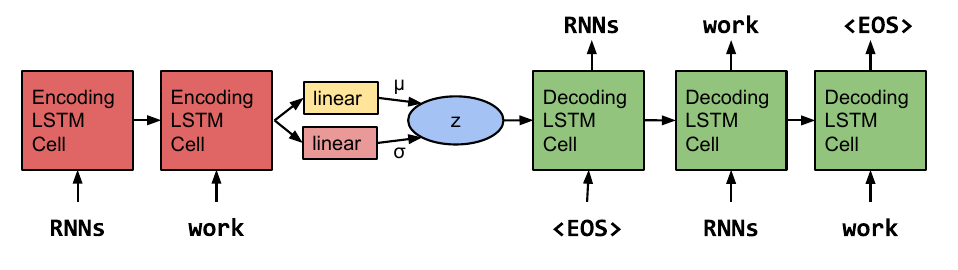
\includegraphics[width=0.5\textwidth]{images/vae-text.png}
	\caption{
		نمایی از مدل \vae{} استفاده شده در حوزه متن
		\cite{vae_text}.}
	\label{fig:vae-text}
\end{figure}
\label{chap2:latent_ignore}
آنچه که در حوزه متن اتفاق می‌افتد، صفر شدن قسمت شامل فاصله \lr{KL}  است؛ در واقع می‌توان این طور بیان کرد که کدگذار بدون توجه به معنی‌دار بودن فضای نهان، هر جمله را مستقلا به یک نقطه از فضای نهان نگاشت می‌کند. در نتیجه‌ی این روند، کدگشا هم مستقل از معنای فضای نهان جمله‌ای را تولید خواهد نمود و توزیع نرمال فرض شده بر فضای نهان یک جمله، چندان حاوی جملات مشابه آن نخواهد بود و روند آموزش به مشکل بر خواهد خورد. \\
یکی از راه‌کارهای اولیه به کار برده شده، دخیل کردن تدریجی قسمت حاوی \lr{KL} به تابع هزینه است. در واقع تابع هزینه به صورت زیر تغییر می‌کند:
\begin{equation}
	\begin{split}
		L_{VAE} = \expected_{\bff{x} \sim p_{data}(\bff{X})} [\lambda_{KL} KL(q(\bff{Z}|\bff{x}) || N(\textbf{\latin{0}},\textbf{\latin{I}}))- \expected_{\bff{z} \sim q(\bff{Z}|\bff{x})}[\log p(\bff{x}|\bff{z})]]
	\end{split}
\end{equation}
که $\lambda_{KL}$ ضریبی مثبت است. در واقع در ابتدا با قرار دادن $\lambda_{KL}=0$، مدل تنها یک خودرمزنگار ساده بوده و فضای نهان معنا داری ساخته و به مرور با میل دادن آن به یک، سعی در جمع کردن فضای نهان در فضای گاوسی نرمال خواهد داشت. جالب توجه است که چنین اتفاقی در حوزه تصویر رخ نمی‌دهد و قسمت \lr{KL} صفر نمی‌شود.
\iffalse
	این پدیده را شاید بتوان این طور توجیه کرد که از یک سو تغییرات ابتدایی فضای نهان زیاد بوده و دخیل کردن این تغییرات در تولید نمونه مورد نظر امری دشوار است؛ از سویی دیگر کدگشا به لحاظ معماری توانایی نگاشت هر نقطه از فضا را به جمله مورد نظر دارد و بنابراین رابطه تولید و استفاده از معنای فضای نهان بین کدگشا و کدگذار چندان شکل نمی‌گیرد.
\fi
گذشته از مشکلات ذکر شده، همان‌طور که در تابع هزینه آن دیده می‌شود همچنان کدگشا سعی در بالابردن درست‌نمایی داده آموزش را داشته و بنابراین این مدل همچنان مشکل \expbias{} را داشته و راه حلی برای این موضوع ارائه نمی‌کند.

به منظور رفع مشکل ذکر شده، کارهای متعددی از جهات مختلف آن را مورد بررسی قرار داده و راه حل‌هایی ارائه داده‌اند. در ادامه تعدادی از آن‌ها توضیح داده خواهند شد.
\subsubsection{عوامل صفر شدن \lr{KL}}
بررسی‌های مختلفی جهت شناسایی عوامل رخداد چنین پدیده‌ای صورت گرفته است که در ادامه به توضیح تعدادی از آن‌ها پرداخته خواهد شد.
\paragraph*{تمایل شبکه \decoder{}
	به استقلال داشتن از فضای نهان}
مقالات متعددی وجود دارند که به تحلیل \vae{} از دیدگاه نظریه اطلاعات پرداخته‌اند. یکی از این دیدگاه‌ها ارتباط روش کدینگ \bitsback{} با \vae{} است \cite{vae_lossy}.\\
فرض کنید بخواهیم اطلاعات را با استفاده از فضای نهان \vae{} کد کنیم. از آنجا که تمام اطلاعات در فضای نهان کد نشده است باید خطای بازسازی را نیز کد کنیم. بنابراین هر کد از دو بخش
$p_\bff{Z}(\bff{Z})$
(\priordist{})
و $p(\bff{X}|\bff{z})$
(توزیع \decoder{})
تشکیل خواهد و میانگین طول کد به شرح زیر است:
\begin{gather}
	\mathcal{L}_{naive} = \expected_{\bff{x} \sim \text{data}, \bff{z} \sim q(\bff{Z}|\bff{x})} [-\log p(\bff{z}) - \log p(\bff{x}|\bff{z})]
\end{gather}
می‌توان روش کدینگ فوق را با استفاده از اطلاعات $q(\bff{z}|\bff{x})$ بهبود داد؛ چراکه این توزیع به طور میانگین حداکثر $H(q(\bff{Z}|\bff{x}))$ اطلاعات در خود دارد. روش به این صورت خواهد بود که \decoder{} هنگام بازگشایی کد، به توزیع تخمینی $\prob(\bff{z}|\bff{x})$ که فرستنده از آن استفاده می‌کند، دسترسی داشته و در نتیجه به اندازه $\log q(\bff{z}|\bff{x})$ از طول کد کم خواهد شد. میانگین طول کد به صورت زیر تغییر خواهد کرد \cite{vae_lossy}.
\begin{gather}
	\mathcal{L}_{\text{BitsBack}} = \expected_{\bff{x} \sim \text{data}, \bff{z} \sim q(\bff{Z}|\bff{x})} [\log q(\bff{z}|\bff{x}) -\log p(\bff{z}) - \log p(\bff{x}|\bff{z})]
\end{gather}
که برابر با تابع هزینه \vae{} است \cite{vae_lossy}:
\begin{gather}
	\begin{align}
		\mathcal{L}_{\text{BitsBack}} = & \expected_{\bff{x} \sim \text{data}} \Big[\expected_{\bff{z} \sim q(\bff{Z}|\bff{x})} [\log p(\bff{x}|\bff{z})] + KL\big(q(\bff{Z}|\bff{x}) ~||~ p(\bff{Z})\big)\Big] \nonumber
		\\
		=                               & \mathcal{L}_{\text{VAE}}
	\end{align}
\end{gather}
از سوی دیگر می‌توان کران پایینی برای تابع هزینه فوق بدست آورد که تابعی از آنتروپی توزیع داده اصلیست. می‌دانیم کران پایین میانگین طول کد برای کد کردن یک نوع داده، آنتروپی آن است. طبق روابط چنین بدست می‌آید \cite{vae_lossy}:
\begin{align}
	\mathcal{L}_{\text{BitsBack}} =
	                                                                           & \expected_{\bff{x} \sim \text{data}, \bff{z} \sim q(\bff{Z}|\bff{x})} [\log q(\bff{z}|\bff{x}) -\log p(\bff{z}) - \log p(\bff{x}|\bff{z})] \nonumber
	\\
	=
	                                                                           & \expected_{\bff{x} \sim \text{data}} [-\log p(\bff{x}) + KL\big(q(\bff{Z}|\bff{x}) ~||~ p(\bff{Z}|\bff{x})\big)] \nonumber
	\\
	\xrightarrow[\text{\lr{by Shannon entropy}}]{\text{\lr{lower bound}}} \geq & \expected_{\bff{x} \sim \text{data}} [-\log p_{\text{data}}(\bff{x}) + KL\big(q(\bff{Z}|\bff{x}) ~||~ p(\bff{Z}|\bff{x})\big)] \nonumber
	\\
	=
	                                                                           & \mathcal{H}(\text{data}) + \expected_{\bff{x} \sim \text{data}} [KL\big(q(\bff{Z}|\bff{x}) ~||~ p(\bff{Z}|\bff{x})\big)]
\end{align}
بنابراین این روش کدینگ به اندازه
$KL\big(q(\bff{Z}|\bff{x}) ~||~ p(\bff{Z}|\bff{x})\big)$
از کدینگ بهینه فاصله دارد و هر قدر این فاصله کمینه گردد، کدینگ نیز طبیعتا بهینه‌تر خواهد بود. \\
اما رابطه فوق چه کمکی به تحلیل پدیده صفر شدن \lr{KL} می‌کند؟ فرض کنید که \decoder{}
($p(\bff{x}|\bff{z})$)
تابعی با قدرت مدل‌سازی بینهایت بوده و توانایی مدل کردن $p_{\text{data}}(\bff{x})$ را مستقل از $\bff{z}$ دارد. از سوی دیگر این امکان برای $q(\bff{z}|\bff{x})$ وجود دارد تا بر خلاف خواسته ما، ضمن عدم استفاده مفید از $\bff{x}$ توزیعی صرفا برابر با $p(\bff{z})$ بسازد. در نتیجه می‌توان با این گونه مدلسازی با آنکه نه $q$ اطلاعات مفیدی را کد کرده و نه $p(\bff{x}|\bff{z})$ از فضای نهان به درستی استفاده می‌کند، از هزینه اضافی
$KL\big(q(\bff{Z}|\bff{x}) ~||~ p(\bff{Z}|\bff{x})\big)$
جلوگیری کرده و به کدینگ بهینه نزدیک شد. این سناریو دقیقا همان اتفاقی است که احتمال وقوع آن در هنگام استفاده از \decoder{} با ساختار \autoregressive{} وجود دارد. برای مثال در صورت استفاده از ساختار \lstm{} (که در تئوری توانایی مدل کردن هر توزیعی را دارد)، \decoder{} می‌تواند بدون استفاده از فضای نهان، توزیع داده اصلی را مدل کند و در نتیجه رابطه موثری بین \decoder{} و \encoder{} شکل نگرفته و 
$KL\big(q(\bff{Z}|\bff{x}) ~||~ p(\bff{Z}|\bff{x})\big)$
صفر شود. به عنوان یک گزاره کلی چنین می‌توان گفت که \decoder{} به اندازه‌ای که بتواند، اطلاعات داده را به صورت محلی مدل کند این کار را انجام داده و هر آنچه که امکان مدلسازی آن به صورت محلی نباشد و یا به عبارت دیگر مربوط به ویژگی‌های کلی یک نمونه باشد، در فضای نهان کد نموده و از آن استفاده می‌کند \cite{vae_lossy}.
\\
با استفاده از تحلیل فوق می‌توان به این نتیجه رسید که چون \vae{} با معماری 
\trans{شبکه‌های عصبی پیچشی}{Convolutional Neural Networks (CNN)}
 در حوزه تصویر، ساختاری  غیر \autoregressive{} دارد، بدون استفاده از فضای نهان، چندان توانایی کم کردن خطای بازسازی را نداشته و مجبور به استفاده از فضای نهان خواهد بود؛ در نتیجه مشکلی که در مدل‌های متنی به وجود می‌آید، در حوزه تصویر با این معماری گزارش نشده است. به طور کلی هر مقدار معماری مورد استفاده توانایی مدل‌سازی محلی کمتری داشته باشد، کمتر مشکل وجود خواهد داشت. توانایی مدل‌سازی محلی را در معماری \cnn{} می‌توان به کم کردن \receiptivefield{} و در \lstm{} به حذف بعضی از کلمات ورودی تعبیر نمود \cite{vae_lossy, vae_dialated, vae_hybrid}.
\paragraph*{بهینه‌های سراسری نامطلوب}
همان ‌طور که در بخش قبل توضیح داده شد، با تطبیق دادن روش کدینگ  \lr{Bits-Back} با مدل \vae{}، می‌توان به این نتیجه رسید که \decoder{} برای رسیدن به میانگین طول کد کمینه، تمایل به استفاده نکردن از فضای نهان دارد. علاوه بر این موضوع، می‌توان نقاطی را یافت که \lr{ELBO} کمینه گردد و از فضای نهان نیز استفاده نگردد \cite{infovae}. می‌دانیم رابطه زیر برای \lr{ELBO} برقرار است:
\begin{align}
	\mathcal{L}_{\text{ELBO}} = & \expected_{\bff{x} \sim p_\text{data}, \bff{z} \sim q(\bff{Z}|\bff{x})} [- \log p_\theta(\bff{x}|\bff{z}) + KL\big(q_\phi(\bff{Z}|\bff{x}) ~ || ~ p(\bff{Z})\big)] \nonumber
	\\
	=                           & \expected_{\bff{x} \sim p_\text{data}} [-\log p_\theta(\bff{x}) + KL\big(q_\phi(\bff{Z}|\bff{x}) ~||~ p_\theta(\bff{Z}|\bff{x})\big)] \nonumber
\end{align}

فرض کنید $p_\theta(\bff{x}|\bff{z})$ وجود داشته باشد که بتواند توزیع داده اصلی را یاد بگیرد؛ به عبارت دیگر، $\theta$ای وجود داشته باشد که $p_\theta(\bff{x}|\bff{z}) = p^*(\bff{x})$. با داشتن این فرض،
$p_\theta(\bff{x}) = p^*(\bff{x})$
و
$p_\theta(\bff{z}|\bff{x})$
برابر با \priordist{} خواهد شد \cite{infovae}:
\begin{gather}
	p_\theta(\bff{X}) = \int_\bff{z} p(\bff{z}) p_\theta(\bff{X}|\bff{z})  = \int_\bff{z} p(\bff{z}) p^*(\bff{X}) = p^*(\bff{X}) \int_\bff{z} p(\bff{z}) = p^*(\bff{X})
	\\
	p_\theta(\bff{Z}|\bff{x}) = \frac{p_\theta(\bff{x}|\bff{Z}) p(\bff{Z})}{p_\theta(\bff{x})} = \frac{p^*(\bff{x}) p(\bff{Z})}{p^*(\bff{x})} = p(\bff{Z})
\end{gather}
حال $q_\phi(\bff{z})$ می‌تواند به سمت $p(\bff{z})$ رفته تا عبارت \lr{KL} بین \posterior{} واقعی و تخمینی صفر گردد. از سوی دیگر هم \likelihood{} بیشینه مقدار خود را دارد ($p_\theta(\bff{x}) = p^*(\bff{x})$) و در نتیجه این حالت یک حالت بهینه سراسری است. از آنجا که $q_\phi(\bff{z}|\bff{x})$ به $p(\bff{z})$ تبدیل شده است، بنابراین رابطه‌ای بین $\bff{x}$ و $\bff{z}$ تحت $q_\phi(\bff{z}|\bff{x})$ وجود نداشته و به عبارت دیگر فضای نهان معنای مطلوب را نداشته گرچه که به بهینه سراسری رسیده‌ایم \cite{infovae}.
\paragraph*{عقب ماندن شبکه
	\encoder{}
	در تخمین توزیع پسین واقعی}
از زاویه‌ای دیگر نیز می‌توان این پدیده را مورد بررسی قرار داد. فروپاشی توزیع \posterior{} به زبان ریاضی به حالتی از مدل اطلاق می‌گردد که
$q_\phi(\bff{z}|\bff{x}) = p_\theta (\bff{z}|\bff{x}) = p(\bff{z})$
است \cite{vae_lagging}. این حالت را می‌توان به دو زیر حالت تقسیم کرد؛ حالت $p_\theta(\bff{z}|\bff{x}) = p(\bff{z})$ و حالت $q_\phi(\bff{z}|\bff{x}) = p(\bff{z})$ که آن‌ها را به ترتیب فروپاشی مدل و فروپاشی استنتاج می‌نامیم. با توجه به این تقسیم بندی می‌توان آزمایشی را ترتیب داد تا متوجه شد کدام حالت موجب چنین رخدادی می‌گردد. به این منظور میانگین دو توزیع $p_\theta(\bff{z}|\bff{x})$ و $q_\phi(\bff{z}|\bff{x})$ که به ترتیب با $\mu_{\bff{x},\theta}$ و $\mu_{\bff{x},\phi}$ نمایش داده می‌شوند را در حین آموزش بررسی و رسم می‌کنیم. هر نقطه $x$ با استفاده از توزیع‌های حاصل از شبکه‌های \encoder{} و \decoder{} به فضای
$(\mu_{\bff{x},\phi}, \mu_{\bff{x},\theta})$
برده شده و سپس نموداری به شکل زیر رسم می‌گردد:
\begin{figure}[H]
	\centering
	\includegraphics[width=0.5\textwidth]{images/lagging1.pdf}
	\caption
    [نموداری بر فضای میانگین توزیع پسین $(\mu_{x,\phi}, \mu_{x,\theta})$.]
    {
		نموداری بر فضای میانگین توزیع پسین $(\mu_{x,\phi}, \mu_{x,\theta})$. محور افقی میانگین توزیع \posterior{} مدل و محور عمودی میانگین توزیع \posterior{} تخمینی را نشان می‌دهد. خط چین قطری نیز حالتی را نشان می‌دهد که میانگین توزیع \posterior{} مدل (واقعی) با تخمینی یکسان شده است \cite{infovae}.
	}
\end{figure}

از آنجا که میانگین \priordist{} برابر صفر است، بنابراین اگر $\mu_{\bff{x},\phi} = 0$ شود فروپاشی استنتاج و اگر $\mu_{\bff{x},\theta} = 0$ باشد فروپاشی مدل اتفاق افتاده است \cite{infovae}. لازم به ذکر است که بایستی ابعاد $\bff{z}$ به گونه‌ای باشد تا بتوان آن را به صورت کارا محاسبه کرد؛ ازین رو $\bff{z}$ یک عدد یک بعدی در نظر گرفته شده است. محور قطری نیز مربوط به حالتی است که $p_\theta(\bff{z}|\bff{x})$ و $q_\phi(\bff{z}|\bff{x})$ از نظر میانگین بر یکدیگر منطبق بوده و توزیع پسین تخمینی، کار خود را به درستی انجام داده است. مبدا نیز مربوط به حالت بهینه محلیِ فروپاشی \posteriordist{} است؛ این در حالی است که احتمالا نقاط بهینه محلی مطلوب‌تر جایی بر روی محور قطری و در اطراف مبدا خواهند داشت.
نمودار‌های زیر حاصل انجام این آزمایش در روند آموزش است.

\begin{figure}[H]
	\centering
	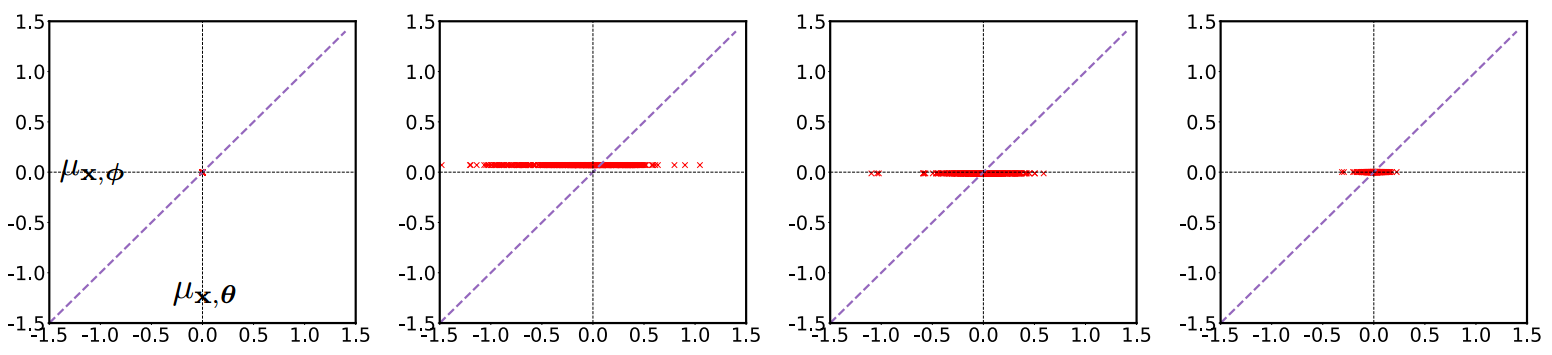
\includegraphics[width=1.\textwidth]{images/lagging2.png}
	\caption
    [مشاهده‌ای از نحوه رخداد حالت فروپاشی استنتاج]
    {
        مشاهده‌ای از نحوه رخداد حالت فروپاشی استنتاج. نمودارهای فوق از تصویر کردن ۵۰۰ نقطه از داده اصلی بر فضای نهان (در ۴ مقطع زمانی. به ترتیب از شکل سمت چپ به راست، گام آموزشی ۰ ام، ۲۰۰ ام، ۲۰۰۰ ام و انتهایی) بدست آمده است. آنچه که در تصویر فوق مشخص است، آن است که در ابتدای آموزش، دو متغیر $\bff{z}$ و $\bff{x}$ از یکدیگر مستقل بوده و در روند آموزش نیز شبکه \encoder{} تخمین صحیحی از \posteriordist{} نداشته و در نتیجه باعث ایجاد حالت فروپاشی استنتاج می‌شود.
	}
\end{figure}
آن طور که از تصاویر برداشت می‌شود به این صورت است که ابتدا نقاط به صورت متمرکز در مبدا جمع شده‌اند اما در ادامه، نقاط در محور افقی گسترده شده‌اند و در انتها مجددا به سمت متمرکز شدن پیش رفته اند. نکته قابل توجه این است که در تمامی این حالات نقاط در محور افقی پراکنده شده‌اند \cite{infovae}. برای توجیه این مشاهده می‌توان از صورت دیگری از رابطه \lr{ELBO} بهره برد. می‌دانیم \lr{ELBO} برابر با عبارت زیر است \cite{vae, vae_lagging}:
\begin{gather}
	\mathcal{L}_{\text{ELBO}}(\bff{x};\theta, \phi) = \log p_\theta(\bff{x}) - {KL}(q_\phi(\bff{Z}|\bff{x})~||~ p_\theta(\bff{Z}|\bff{x}))
\end{gather}
که عبارت اول مربوط به \likelihood{} حاشیه‌ای و عبارت دوم مربوط به فاصله توزیع تخمینی $q_\phi(\bff{z}|\bff{x})$ از توزیع پسین واقعی مدل ($p_\theta(\bff{z}|\bff{x})$) است. واضح است که پارامتر $\phi$ تنها تحت تاثیر عامل \lr{KL} بوده در حالی که پارامتر $\theta$ علاوه بر این، تحت تاثیر عبارت \likelihood{} حاشیه‌ای نیز هست. علاوه بر این تنها عاملی که باعث ایجاد رابطه بین $\bff{x}$ و $\bff{z}$ می‌گردد،
\likelihood{}
است و بخش دوم تنها سعی در نزدیک کردن دو توزیع $p_\theta(\bff{z}|\bff{x})$ و $q_\phi(\bff{z}|\bff{x})$ دارد \cite{infovae}.

حال با نگاه داشتن به رابطه فوق، این پدیده را این طور می‌توان تفسیر نمود که با وجود اینکه ابتدا فضای نهان ساخته شده تقریبا مستقل از فضای داده‌های ورودی است، با پراکنده شدن نقاط به صورت افقی در ادامه روند آموزش، رابطه‌ای بین $\bff{z}$ و $\bff{x}$ تحت مدل $p_\theta(\bff{x})$ در حال شکل‌گیری است؛ اما به دلیل اینکه شبکه \encoder{} به هیچ عنوان تخمین صحیحی از \posteriordist{} واقعی ندارد و همزمان در حال کمینه کردن هر دو قسمت عبارت \lr{ELBO} نسبت به پارامترهای هر دو شبکه‌ی \encoder{} و \decoder{} هستیم، در نتیجه با ادامه آموزش، رابطه بین این دو متغیر به مرور بر اثر غلبه بخش حاوی فاصله \lr{KL} بر بخش \likelihood{} حاشیه‌ای، از دست رفته و سیستم دچار یک بهینه محلی می‌گردد \cite{infovae}.

\subsection{مدل‌های ارائه شده برای رفع مشکل صفر شدن \lr{KL}}
به طور کلی راه حل‌های ارائه شده یا از جنس تغییر معماری ‎\decoder{}‎ و ضعیف کردن قدرت ‎\autoregressive{}‎ آن، تغییر ‎\priordist{}‎ و یا تغییر تابع هزینه هستند. در ادامه به توضیح برخی از این روش‌ها پرداخته خواهد شد.
\subsubsection{استفاده از \cnn{} به جای \lstm{} در \decoder{}}
\begin{figure}[h]
	\centering
	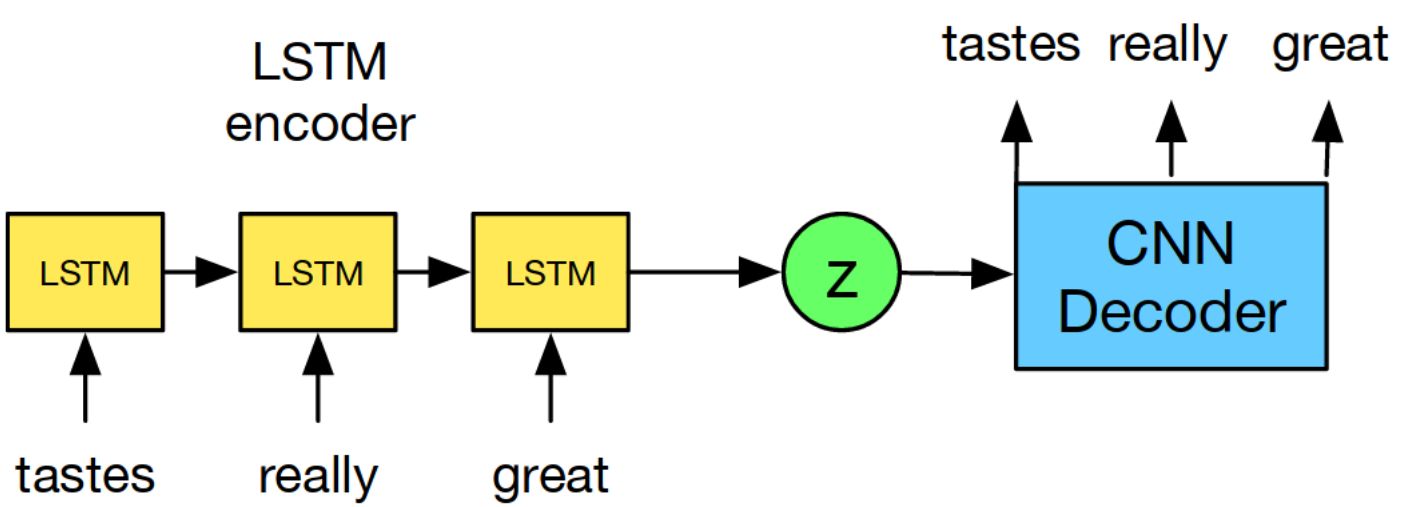
\includegraphics[width=0.5\textwidth]{images/dialated-conv1.png}

	\vspace{0.5cm}

	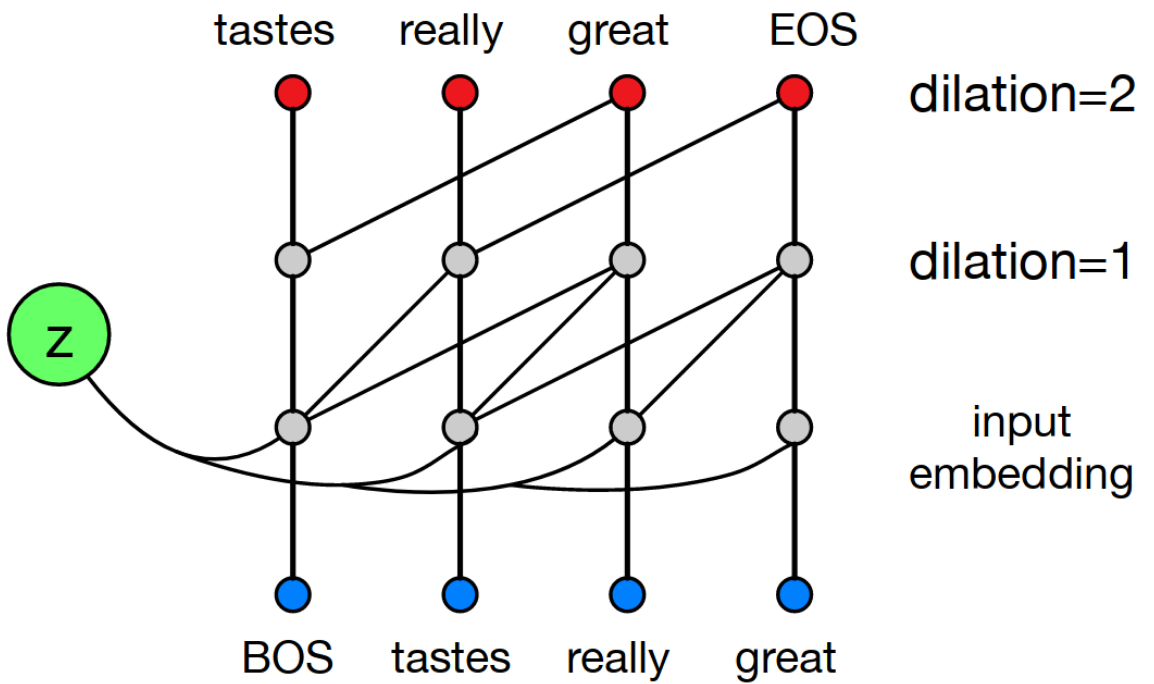
\includegraphics[width=0.5\textwidth]{images/dialated-conv2.png}
	\caption{
		معماری کلی شبکه ارائه شده که از \cnn{}  با کانولوشن‌های \dilated{} در  ‎\decoder{}‎ بهره می‌برد.
	}
	\label{fig:dialted_conv}
\end{figure}
راه حل‌های اولیه بیشتر در حوزه تغییر ساختار ‎\decoder{}‎ هستند. دلیل چنین رویکردی در این بود که می‌توان مشکل را در قدرت زیاد مدل‌های ‎\lstm{} در مدلسازی به صورت ‎\autoregressive{}‎ جست و جو کرد \cite{vae_dialated}؛ چراکه در حوزه تصویر که هر پیکسل مستقل از سایر پیکسل‌ها تولید می‌گردد، چنین پدیده‌ای گزارش نشده است. بنابراین یک راه حل استفاده از مدل‌هایی است که قدرت \autoregressive{} کمتری دارند. برای مثال همان طور که در شکل ‎\ref{fig:dialted_conv}‎ نشان داده شده است، می‌توان ‎\decoder{}‎ را با وام گرفتن از ایده شبکه ‎\lr{PixelCNN}‎ با معماری ‎\cnn{}‎ پیاده‌سازی و جایگزین ‎\lstm{}‎ نمود. به طور دقیق‌تر برای پیشبینی هر پیکسل، پیکسل‌های پیش‌رو پوشانده شده، از فیلتر‌های یک بعدی و اتصالات
\trans{انبساطی}{Dilated}
در کانولوشن‌ها بهره گرفته شده که در نتیجه
\trans{حوزه تاثیر}{Receiptive field}
در هر لایه نسبت به لایه قبل، افزایش نمایی پیدا کند \cite{vae_dialated}. در واقع با زیاد شدن تعداد لایه‌های با کانولوشن‌های \dilated{}، 
\trans{زمینه}{Context}
 طولانی‌تری در خروجی یک گره از لایه مورد نظر دخیل خواهد شد. برای مثال اگر ضریب انبساط ۲ استفاده گردد، \receiptivefield{}‎ در هر لایه نسبت به لایه قبل تقریبا دو برابر شده و در نتیجه از آنجا که می‌بایست کلمه آخر جمله تابعی از تمام کلمات پیشین باشد،‌ نیاز به $‎\log T$ لایه خواهد بود که $T$ طول بلندترین جمله است. ادعای مقاله بر اساس آزمایش‌های متفاوت بر این است که ساختار \cnn{} بیشتر متکی بر فضای نهان  $Z$ بوده و بنابراین مشکل ذکر شده را مقداری تقلیل می‌دهد. نکته قابل ذکر این است که در این حالت نیز اگر ‎اندازه شبکه بسیار بزرگ شود مجددا مشکل صفر شدن ‎\lr{KL}‎ ظهور پیدا می‌کند \cite{vae_dialated}.

\subsubsection{\aae{}
    \protect\LTRfootnote{Adversarial autoencoder (AAE)}
} \label{sec:aae}
مدل \aae{}، نسخه تغییر یافته‌ای از مدل \vae{} است تا بخشی از ضعف‌های آن را بپوشاند. همان طور که قبلا نیز توضیح داده شد، تابع هزینه \vae{} از دو بخش تشکیل شده است. بخش اول مربوط به کمینه کردن خطای بازسازی و بخش دوم مربوط به سوق دادن فضای نهان به توزیع گاوسی نرمال است. مدل \aae{}، با حفظ بخش مربوط به خطای بازسازی، در بخش دوم به جای نزدیک کردن توزیع خروجی ‎\encoder{}‎ به  ‎‎\priordist{‎}‎
($q(\bff{z}|\bff{x}) ‎\leftrightarrow p(\bff{z})$)،
سعی در نزدیک کردن توزیع 
\trans{حاشیه‌ای}{Marginal}
خروجی  ‎\encoder{‎}‎  را  به \priordist{} مورد نظر دارد
($q(z) ‎\leftrightarrow  p(z)$) \cite{aae}.
در واقع توزیع \marginal{} $q(\bff{z})$ به صورت زیر تعریف می‌شود:
\begin{gather}
	q(Z) = \sum_\bff{x} p_{data}(\bff{x}) q(\bff{Z}|\bff{x})
\end{gather}
و هدف نزدیک کردن توزیع $q(\bff{z})$ به $p(\bff{z})$ خواهد بود \cite{aae}. بنابراین در مقایسه با مدل \vae{}، اجازه داده می‌شود تا به جای اینکه خروجی \encoder{} به ازای هر نمونه، مستقل از سایر نمونه‌ها به یک توزیع گاوسی نرمال نزدیک شود، توزیع ‎\marginal{}‎ نمونه‌های داده واقعی در فضای نهان، یک توزیع نرمال گاوسی باشد.
\begin{figure}[H]
	\centering
	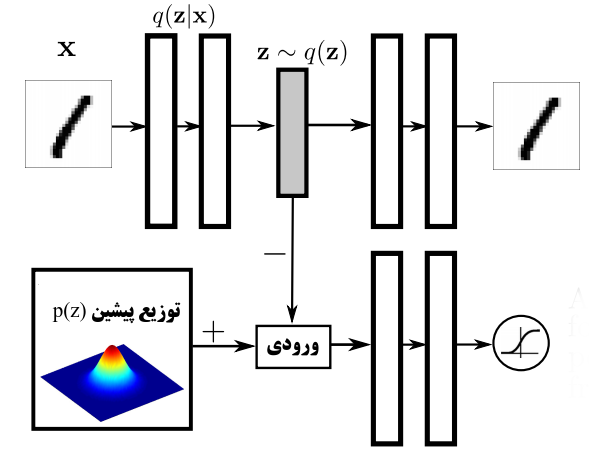
\includegraphics[width=.6\textwidth]{images/aae.png}
	\caption
    [نمایی از مدل  \aae{}.]
    {
		نمایی از مدل  \aae{}. در واقع این مدل، همان مدل \autoencoder{} است که بخش منظم‌ساز مربوط به نزدیک کردن $q(\bff{z})$ به $p(\bff{z})$ به آن افزوده شده است \cite{aae}. برای نزدیک کردن این دو توزیع نیز از رویکرد \gan{} استفاده شده که نمونه‌های \priordist{} نمونه‌های مثبت و نمونه‌های تولید شده توسط \encoder{} نمونه‌های منفی تلقی شده و داده ورودی شبکه \discriminator{} می‌سازند.
	}
	\label{fig:aae}
\end{figure}
گفته شد که بایستی دو توزیع $p(\bff{z})$ و $q(\bff{z})$ به یکدیگر نزدیک شوند. حال بر خلاف آنچه که در مدل \vae{} اتفاق می‌افتاد که بخش $KL$ نیاز به محاسبه به صورت فرم بسته داشت، با وام‌گیری از ایده \gan{}، می‌توان \discriminator ‌ای آموزش داد تا نمونه‌های \priordist{} را از نمونه‌های توزیع \marginal
$q(\bff{z})$
جدا کند. در واقع اگر بخواهیم با ادبیات شبکه‌های تخاصمی معادل‌سازی کنیم، مولد $q(\bff{z})$ و توزیع داده واقعی $p(\bff{z})$ خواهد بود که نمایی از این روش نیز در شکل \ref{fig:aae} آمده است. رابطه تابع هزینه این مدل به شکل زیر است \cite{aae}:
\begin{gather}
	L_{AAE}(\phi, \theta) =
	- \expected_{\bff{x} \sim p_{data}, \bff{z} \sim q_\phi(\bff{Z}|\bff{x})} [\log (D(\bff{z}))]
	+ \expected_{\bff{x} \sim p_{data}, \bff{z} \sim q_\phi(\bff{Z}|\bff{x})}[\log p_\theta(\bff{x}|\bff{z})]\\
	L_{AAE}(D) =
	- \expected_{\bff{z} \sim p(\bff{Z})} [\log D(\bff{z})]
	- \expected_{\bff{x} \sim p_{data},\bff{z} \sim q_\phi(\bff{Z}|\bff{x})} [\log (1 - D(\bff{z}))]
\end{gather}
که $q_\phi(\bff{z}|\bff{x})$ توزیع \encoder{}،
$p_\theta(\bff{x}|\bff{z})$
توزیع \decoder{} و $p(\bff{z})$ توزیع پیشین است. روند بهینه‌سازی به این صورت است که مانند \gan{} از دو بخش تشکیل شده است؛ بخش بهینه‌سازی خطای بازسازی و بخش تخاصمی. در بخش خطای بازسازی، تنها \autoencoder{} به منظور کاهش خطای بازسازی آموزش داده می‌شود و در بخش تخاصمی، ابتدا \discriminator{} به منظور جداسازی نمونه‌های واقعی از مصنوعی و سپس \encoder{} به منظور نزدیک کردن توزیع \marginal{}‎ فضای نهان به \priordist{} آموزش داده می‌شود \cite{aae}.\\
نکته دیگری که می‌توان در نحوه آموزش مدل به آن اشاره نمود این است که کافیست تا بتوانیم از دو توزیع پیشین و حاشیه‌ای \encoder{} نمونه‌برداری کنیم و مانند مدل \vae{}، نیازی به داشتن فرم بسته رابطه بالا نیست که از مزیت‌های این مدل به شمار می‌رود؛ اما از سوی دیگر این مدل بدون پشتوانه نظری و بررسی رابطه آن با \likelihood{} ارائه شد.\\
در مورد نحوه عملکرد ‎\encoder{}‎ چندین گزینه وجود دارد:
\begin{itemize}
	\item \textbf{\deterministic{}:}
	      در اینجا، $q(\bff{z}|\bff{x})$ یک تابع قطعی از $x$ بوده و تنها عامل تصادفی بودن توزیع  $q(\bff{z})$، توزیع داده واقعی $p_{data}‎(\bff{x})$ است \cite{aae}.
	\item \textbf{توزیع \posterior{} گاوسی:}
	      می‌توان خروجی ‎\encoder{}‎ را توزیع گاوسی با ماتریس کوواریانس قطری در نظر گرفت. بنابراین دو عامل تصادفی در $q(\bff{z})$ وجود خواهد داشت؛ توزیع داده اصلی و توزیع خروجی ‎\encoder{}‎ . به منظور آموزش مدل مشکلات مشابه آموزش ‎\vae{}‎ وجود دارد که مجددا می‌توان از ترفند ‎\reparametrization{}‎ بهره برد \cite{aae}.
	\item \textbf{
        \trans{تخمین‌گر عمومی}{Universal approximator}
         توزیع \posterior{}:}
	      این حالت، کلی‌ترین حالت ممکن برای ‎‎\encoder{}‎ است. ‎\encoder{}‎ به این صورت عمل می‌کند که با گرفتن نویز $‎‎\eta$ (با داشتن توزیع از قبل تعریف شده) و نمونه $\bff{x}$، یک $\bff{z}$ در فضای نهان تولید می‌کند. در واقع ‎\encoder{}‎ یک تابع قطعی از $\bff{x}$ و $‎\eta$ است. مانند حالت قبل، دو عامل تصادفی وجود دارد؛ توزیع داده اصلی و توزیع نویز اولیه. اما بر خلاف مدل قبل، خروجی ‎\encoder{}‎ ، توزیع از پیش تعیین شده‌ای نداشته و با پارامترهای ‎شبکه \encoder{}‎ پارمتری می‌شود. در این حالت $q(\bff{z})$ به شکل زیر خواهد بود:
	      \begin{gather}
		      q(\bff{z}) = \sum_\bff{x} q(\bff{z}|\bff{x}) p_{data}(\bff{x}) = \sum_\bff{x} \sum_\eta p_{data}(\bff{x}) p(\eta)  q(\bff{z}|\bff{x}, \eta)
	      \end{gather}
\end{itemize}
لازم به ذکر است که در دو حالت آخر، ‎با داشتن دو عامل تصادفی، احتمالا توزیع  ‎\marginal{}‎ ‎\encoder{}‎ ، توزیعی با تغییرات  نَرم‌تر خواهد بود \cite{aae}.
\subsubsection{\wae} \label{chap2:wae}
مدل \wae{} که در ادامه معرفی خواهد شد، نسخه عمومی‌تر مدل \aae{}‎ بوده که به لحاظ تئوری نیز بررسی گردیده است.\\
در بخش ‎\ref{sec:aae}‎ توضیح داده شد که تفاوت ‎\aae{}‎ با مدل ‎\vae{}‎، در نحوه اعمال توزیع مورد نظر بر فضای نهان است. با تکیه بر همین نکته، حالت کلی‌تری از ‎\aae{}‎ به نام ‎\wae{}‎ ارائه شد. در واقع همان طور که در شکل ‎‎\ref{fig:wae}‎ مشخص است، در ‎\vae{}‎ توزیع خروجی \encoder{} به ازای هر نمونه به ‎\priordist{}‎ نزدیک می‌شود. در نتیجه این عمل، خروجی \encoder{} به ازای نمونه‌های متفاوت مجبور به داشتن همپوشانی خواهد شد؛ بنابراین بازسازی نمونه‌های داده اصلی از فضای نهان با مشکل مواجه خواهد شد. در مقابل، در ‎\wae{}‎ مقداری دست مدل در نحوه اعمال ‎‎\priordist{}‎ به فضای نهان باز بوده و تنها کافیست توزیع ‎\marginal{}‎ حاکم بر فضای نهان دارای ‎\priordist{}‎ باشد \cite{wae}.\\
\begin{figure}[H]
	\centering
	\begin{subfigure}[b]{0.4\textwidth}
		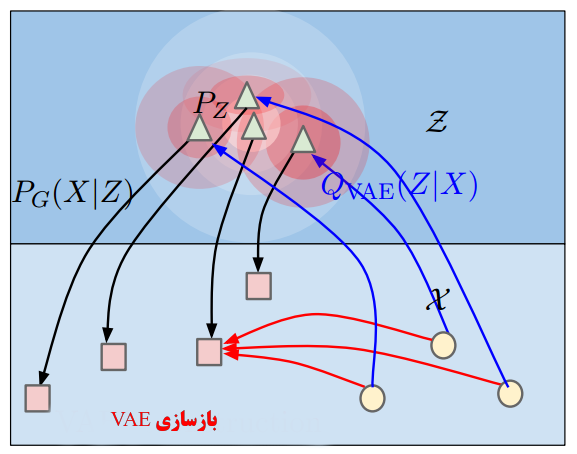
\includegraphics[width=\textwidth]{images/wae1.png}
		\caption{\vae}
		\label{fig:wae-vae}
	\end{subfigure}
	\begin{subfigure}[b]{0.4\textwidth}
		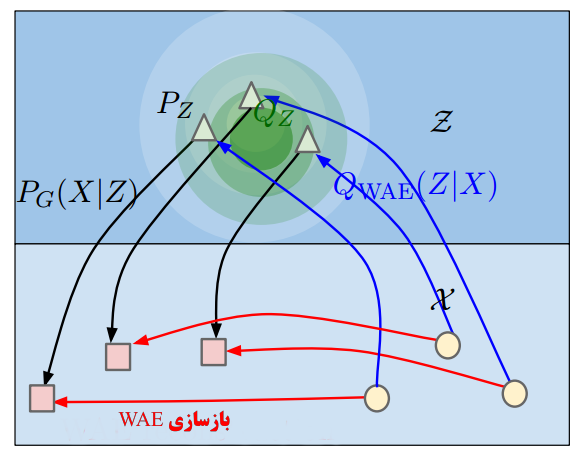
\includegraphics[width=\textwidth]{images/wae2.png}
		\caption{\wae}
		\label{fig:wae-wae}
	\end{subfigure}
	\caption
    [مقایسه نحوه بازسازی در مدل  ‎‎\wae{}‎ با ‎\vae{}‎.]
    {
		مقایسه نحوه بازسازی در مدل  ‎‎\wae{}‎ با ‎\vae{}‎. دوایر قرمز رنگ در فضای نهان مربوط به توزیع (گاوسی) خروجی ‎\encoder{}‎، دوایر سبز رنگ مربوط به توزیع ‎‎\marginal{}‎ خروجی ‎\encoder{}‎ و  دوایر سفید رنگ، متناظر با ‎\priordist{}‎ (گاوسی نرمال) است. همان طور که در شکل ‎\subref{fig:wae-vae}‎ مشخص است، هر ناحیه قرمز سعی در نزدیک شدن به ناحیه سفید رنگ دارد؛ بنابراین به دلیل وجود همپوشانی بین نواحی مختلف قرمز، مشکلاتی در بازسازی پیش خواهد آمد. این در حالیست که در مدل ‎\wae{}‎ ، تمرکز بر اعمال توزیع گاوسی بر توزیع ‎\marginal{}‎ \encoder{}‎‎ است \cite{wae}.
	}
	\label{fig:wae}
\end{figure}
بر خلاف آن که در روش ‎\aae{}‎ اظهار نظری راجع به رابطه تابع هزینه معرفی شده و ‎\likelihood{}‎ مدل ارائه نشد، مدل ‎\wae{}‎ به بررسی این موضوع پرداخته است.
مدل گرافی در نظر گرفته شده برای این روش مانند مدل گرافی ‎\vae{}‎ است. متغیر نهان $\bff{z}$ ای با توزیعی مشخص و ثابت وجود دارد که نمونه $\bff{x}$ از آن بدست خواهد آمد. اگر ‎\priordist{}‎ متغیر نهان را با $p_\bff{Z}(\bff{z})$ و ‎توزیع ‎‎‎\decoder{}‎‎ را با $p_G(\bff{x}|\bff{z})$ نشان دهیم، توزیع ‎\marginal{}‎
$p_G(\bff{x})$
به صورت زیر تعریف می‌شود:
\begin{gather}
	p_G(\bff{X}) = \sum_\bff{z} p_\bff{Z}(\bff{z}) p_G(\bff{X}|\bff{z})
\end{gather}
حال برای اینکه این توزیع را به توزیع $p_{data}‎(\bff{x})$ نزدیک کنیم، از فاصله‌های متعددی می‌توان استفاده نمود \cite{wae}. در اینجا همان طور که از نام مدل بر‌می‌آید، از فاصله ‎‎ \wasser{} بهره برده شده است. اگر فاصله ‎‎\wasser{}‎ با تابع هزینه $c$‎ را با $W_c$ نشان دهیم، اثبات شده است که رابطه $W_c(p_{data}‎, p_G)$ را می‌توان به شرح زیر بازنویسی کرد:
\begin{align}
	\label{eq:wae_constrained}
	W_c(p_{data}, p_G) & = \inf_{\Gamma \in \Pi(p_{data}, \sim p_G)} \expected_{(\bff{x}, \bff{y}) \sim \Gamma} [c(\bff{x}, \bff{y})] \nonumber       \\
	                   & = \inf_{Q: q_z = p_z} \expected_{\bff{x} \sim p_{data}} \expected_{\bff{z} \sim q(\bff{Z}|\bff{x})} [c(\bff{x}, G(\bff{z}))]
\end{align}
که $q_\bff{Z}(\bff{z})$، توزیع ‎\marginal{}‎ فضای نهان است؛ به عبارت دیگر:‌
$q_\bff{Z}(\bff{Z}) = ‎\sum_\bff{x} q(\bff{Z}|\bff{x})p_{data}‎(\bff{x})$
طبق رابطه بالا، به منظور کاهش فاصله ‎\wasser{}‎ بین دو توزیع $p_{Data}‎$ و $p_G$ کافیست توزیع شرطی
$q(\bff{z}|\bff{x})$ای
بیابیم که توزیع ‎\marginal{}‎ آن برابر با توزیع $p_\bff{Z}$ باشد. مشکلی که در رابطه ‎\ref{eq:wae_constrained}‎ وجود دارد این است که مسئله بهینه‌سازی با قید است. به منظور رفع این قید می‌توان آن را به شکل زیر بازنویسی کرد:
\begin{gather}
	V_text{WAE}(q, G) = \inf_{G \in \mathcal{G}, ~ q \in \mathcal{Q}} \expected_{\bff{x} \sim p_{Data}, \bff{z} \sim q(\bff{Z}|\bff{x})} [c(\bff{x}, G(\bff{z}))] + \lambda . D_\bff{Z}(q_\bff{Z}, p_\bff{Z})
\end{gather}
که $‎\mathcal{Q}‎$  و ‎$‎\mathcal{G}$ خانواده توابعی هستند که با شبکه عصبی توانایی مدل کردن آن‌ها را داشته و $D_\bff{Z}(. , .)$ هم می‌تواند هر فاصله‌ای بین دو توزیع $q_\bff{Z}$ و $p_\bff{Z}$ باشد (تنها کافیست بتوان از آن نسبت به پارامترهای شبکه مشتق گرفت)\cite{wae}. لازم به ذکر است که در رابطه بالا، لزومی به تصادفی بودن خروجی ‎\encoder{}‎ نبوده و حالت  ‎\deterministic{}‎ هم می‌تواند داشته باشد.\\
حال اینکه به جای $D_\bff{Z}(. , .)$ از چه معیار یا روشی استفاده گردد، در این مقاله دو گزینه ارائه شده است که بیان خواهند شد:
\begin{itemize}
	\item \textbf{مبتنی بر معماری تخاصمی:}
	      می‌دانیم ‎\gan{}‎‌ها فاصله ‎\lr{JS}‎ را کمینه می‌کنند. به منظور کمینه کردن $D_\bff{Z}(. , .)$ نیز می‌توان از این فاصله بهره برد \cite{wae}. به این صورت که یک شبکه ‎\discriminator{}‎ برای تمیز دادن نمونه‌های ‎\priordist{}‎ از ‎‎نمونه‌های حاصل از خروجی ‎\encoder{}‎ استفاده می‌گردد؛ از سوی دیگر ‎\encoder{}‎ سعی در تولید نمونه‌هایی خواهد داشت که به نمونه‌های ‎\priordist{}‎ نزدیک بوده و ‎\discriminator{}‎ به اشتباه بیفتد. بنابراین اگر \discriminator{} را با $D$ نشان دهیم، توابع هزینه به شکل زیر خواهد بود:
	      \begin{gather}
		      V(q, G)= \inf_{q, G}
		      \expected_{\bff{x} \sim p_{Data}, \bff{z} \sim q(\bff{Z}|\bff{x})} [c(\bff{x}, G(\bff{z}))]
		      - \lambda (\expected_{\bff{x} \sim p_{Data}, \bff{z} \sim q(\bff{Z}|\bff{x})} [\log D(\bff{z})]) \nonumber
		      \\
		      V(D)= \sup_{D}
		      \expected_{\bff{x} \sim p_{Data}, \bff{z} \sim q(\bff{Z}|\bff{x})} [\log (1-D(\bff{z}))]
		      + \expected_{\bff{z} \sim p(\bff{Z})} [\log D(\bff{z})]
	      \end{gather}
	\item \textbf{مبتنی بر فاصله \mmd :}
	      همان طور که در بخش \ref{chap2:divs} توضیح داده شد، اگر تابع کرنل $k$ ویژگی‌های مشخصی را داشته باشد، ‎\mmd{}‎ را به یک متر تبدیل کرده و این امکان را فراهم می‌کند تا از این متر به عنوان تابع هزینه برای کمینه کردن فاصله $p_\bff{Z}$  و $q_\bff{Z}$  بهره برده شود. از آنجا که رابطه بالا به طور مستقیم قابل محاسبه و بهینه‌سازی نیست، از تخمین‌گر نااریب زیر استفاده می‌گردد \cite{wae}. اگر $n$ نمونه از دو توزیع $p_\bff{Z}$  و $q_\bff{Z}$ داشته و به ترتیب با $\bff{z}_i$ و $‎\tilde{\bff{z}}_i$ نشان داده شوند،‌خواهیم داشت:

   \begin{align}
    \mathsf{MMD}_k(\bff{z}{1,2,...,n};\tilde{\bff{z}}_{1,2,...,n}) = & \frac{1}{n(n-1)} \sum_{l \neq j} k(\bff{z}_l, \bff{z}_j) +
    \frac{1}{n(n-1)} \sum_{l \neq j} k(\tilde{\bff{z}}_l, \tilde{\bff{z}}_j)                                               \nonumber          \\
                                                                     & - \frac{1}{n ^ 2} \sum_{l, j} k(\bff{z}_l, \tilde{\bff{z}}_j)
   \end{align}

\end{itemize}‎
بدست آمدن نمونه از توزیع $p_\bff{Z}$ واضح است و برای نمونه‌برداری از توزیع $q_\bff{Z}$ نیز با استفاده از روش
\trans{سلسله مراتبی}{Ancestral}
ابتدا از توزیع $p_{data}‎$ نمونه‌برداری کرده و سپس از توزیع $q(\bff{z}|\bff{x})$ نمونه‌برداری انجام می‌گیرد.
نکته قابل ذکر این است که قضایای ارائه شده تنها در حالتی که ‎\decoder{}‎ تابعی قطعی باشد صادق هستند؛ البته قضیه مشابهی برای \decoder{} با خروجی تصادفی، اما تنها در حالتی که از تابع هزینه مجذور فاصله استفاده می‌شود، ارائه شده است \cite{wae}.
\subsubsection{
    مدل \autoencoder{} منظم‌شده تخاصمی (\lr{ARAE})
\protect\LTRfootnote{Adversarially Regularized Autoencoder (ARAE)}
} \label{chap2:arae}
این مدل با اینکه قبل از \wae{} منتشر شده است، اما در واقع مربوط به استفاده از \wgan{} و \wae{} در حوزه متن است. در بخش قبل در حالت کلی توضیح داده شد که تابع هزینه \wae{} به صورت زیر است:
\begin{align}
	\mathcal{L}_{\text{WAE}}(q, G) = \expected_{\bff{x} \sim p_{\text{Data}}}\expected_{\bff{z} \sim q(\bff{Z}|\bff{x})} [c(\bff{x}, G(\bff{z}))] + \lambda . D_ \bff{Z}(q_\bff{Z}, p_\bff{Z})
\end{align}
در این مقاله، دو موضوع بررسی شده است. موضوع اول استفاده از تابع هزینه \crossentropy{} به جای $c(.,.)$ بوده و دوم نیز استفاده از \wgan{} به عنوان $D_\bff{Z}(.,.)$ به طوری که مناسب فضای تولید دنباله و متن باشد \cite{wae_text_reg}.
\\
فرض کنید $\mathcal{X} = \mathcal{V}^n$ فضای بردارهای
\trans{تک یک}{One-hot}
به طول $|\mathcal{V}|^n$ باشد که $\mathcal{V}$ مجموعه واژگان و $n$ نیز حداکثر طول جملات است (هر بردار متناظر با یک جمله است). همچنین تابع \encoder{} و \decoder{} به ترتیب به صورت
$\text{enc}_\phi: \mathcal{X} \rightarrow \mathcal{Z}$
که تابعی قطعی است و $f_\psi(\bff{Z}) : \mcal{Z} \rightarrow \Delta^{|\mcal{V}|^n - 1}$ تابعی از فضای نهان به
\trans{سادک}{Simplex}
 $|\mcal{V}|^n - 1$
بعدی (توزیع شرطی بر روی فضای $\mathcal{X}$) است، تعریف شده‌اند. همچنین
\linebreak
$\hat{\bff{x}} = G_\psi(\bff{Z})  = \argmax_{
		\bff{x}} f_\psi(\bff{x}|\bff{Z}) : \mcal{Z} \rightarrow \mcal{X}$
خروجی \decoder{} در حالت آزمون و توزیع $p_\psi(\bff{x}|\bff{z})$ حاصل از آن توزیعی ضربه‌ای به صورت
$p_\psi(\bff{x}|\bff{z}) = \bbm{1}\{\bff{x} = G_\psi(\bff{z})\}$
باشد، تابع هزینه زیر کران بالایی برای فاصله \wasser{} بین $p_\text{Data}(\bff{x})$ و $p_\psi(\bff{x})$ است که
$p_\psi(\bff{x}) = \int_\bff{z} p_Z(\bff{z})p_\psi(\bff{x}|\bff{z})$
:
\begin{align}
	\mathcal{L}_{\text{ARAE}}(q, G) = \inf_{q: q_z = p_z} \expected_{\bff{x} \sim p_{\text{Data}}}\expected_{\bff{z} \sim q(\bff{Z}|\bff{x})} [-\log \bff{x}^T f_\psi(\bff{z})]
\end{align}
در اینجا نیز به مانند بخش آموزش  \wae{} برای رفع قید ذکر شده از نوعی فاصله به نام \wgan{} استفاده می‌شود \cite{wae_text_reg}.
 \wgan{} نیز عضوی از خانواده \gan{} است که رفتار مناسب‌تری هنگام فاصله زیاد مولد از داده اصلی از خود بروز می‌دهد. این روش به شرح زیر است:
در اینجا نیز یک \generator{} و یک \discriminator{} داریم. البته در ادبیات \wgan{} به \discriminator{}،
\trans{نقاد}{Critic}
گفته می‌شود که وظیفه دارد به نمونه‌های واقعی اعداد بالاتر و به نمونه‌های مصنوعی اعداد پایین‌تری نسبت دهد.
اگر $g_\theta(\bff{\epsilon})$ شبکه‌ای باشد که با گرفتن یک نوفه با توزیع گاوسی نرمال، آن را به نمونه‌ای در فضای نهان تبدیل کند و $f_w(\bff{X})$ یک \critic{} بین نمونه‌های تولید شده توسط مولد ($g$) و داده‌های واقعی باشد، تابع هزینه ذیل استفاده می‌گردد:
\begin{gather}
	\mathcal{L}_\text{WGAN} (g, D)=
	\expected_{\bff{x} \sim p_\text{Data}(\bff{X})} f(\bff{x})
	- \expected_{\bff{x} \sim p_g(\bff{X})} f(\bff{x})
	\\
	\text{\lr{s.t: f is 1-Lipschitz}} \nonumber
\end{gather}
که نسبت به $w$ بیشینه و نسبت به $\theta$ کمینه می‌گردد \cite{wgan}. در واقع تابع هزینه فوق فاصله \wasser{} بین دو توزیع $p_g(\bff{X})$ و $p_\text{Data}(\bff{X})$ است. برای برآوردن شرط \lr{1-Lipschitz} بودن $f$ نیز از روش ساده قطع کردن گرادیان‌های خارج از بازه $[-m, m]$ استفاده شده است \cite{wae_text_reg}.
\\
در این مقاله نیز برای نزدیک کردن فاصله توزیع حاشیه‌ای $q_\bff{Z}$ با $p_\bff{Z}$ از \wgan{} استفاده شده است. در نهایت تابع هزینه‌های این مدل را می‌توان به شکل زیر جمع‌بندی کرد \cite{wae_text_reg}:
\begin{align}
	\min_{\phi, \psi} \mcal{L}_\text{rec}(\phi, \psi) = & \expected_{\bff{x} \sim p_\text{Data}} [- \log f_\phi(\bff{x}|enc_\phi(\bff{x}))] \nonumber
	\\
	\max_{w} \mcal{L}_\text{critic}(w) =                &
	\expected_{\bff{x} \sim p_\text{Data}} [f_w(\text{enc}_\phi(\bff{x}))]
	-\expected_{\bff{z} \sim p_\bff{Z}} [f_w(\bff{z})] \nonumber
	\\
	\min_{\phi} \mcal{L}_\text{enc}(\phi) =                   &
	\expected_{\bff{x} \sim p_\text{Data}} [f_w(\text{enc}_\phi(\bff{x}))]
\end{align}


آنچه که تا به حال توضیح داده شد، روش‌هایی بودند که به نظر موثرتر و پایه‌ای تر به موضوع پرداخته بودند؛ اما مقالات بسیاری در این حوزه ارائه شده است که در اینجا از آن‌ها صرف نظر شده است \cite{vae_decflow, vae_hybrid, vae_multilevel, vae_spherical}.
\iffalse
\subsubsection{دیگر روش‌های جلوگیری از صفر شدن فاصله \lr{KL}}
\fi
نوع دیگری از مدل‌های مولد موجود است که تا به حال چندان نه در حوزه تصویر و به مراتب بیشتر در حوزه متن مورد توجه قرار نگرفته اند. در ادامه به توضیح این دسته نیز پرداخته خواهد شد.

\section{\condtg}
تا به اینجا به دلیل مشابهت مدل‌های مولد شرطی و غیر شرطی، به معرفی تعدادی از معروف‌ترین مدل‌های مولد غیر شرطی، مشکلات آموزش و راه‌حل‌های رفع آن‌ها پرداخته شد. در این بخش چند مورد مدل مولد شرطی ساده و در ادامه چند مدل شرطی پیچیده‌تر معرفی خواهند شد. در بخش داده را با $\mcal{X} = \{(\bff{x}_n, c_i)\}_{n=1}^N$ نشان می‌دهیم.
\subsection{\rnn{}
     شرطی}
ساده‌ترین رویکردی که در مدل‌های شرطی مورد استفاده قرار می‌گیرد، دخیل کردن شروط مورد نظر به ورودی مولد با ساختار
\trans{شبکه عصبی خودبازگشتی}{Recurrent Neural Network (RNN)}
است. در روش جبر معلم می‌توان شرط را به بردار
\trans{تعبیه}{Embedding}
و  یا در صورت داشتن بردار نهان، به انتهای بردار نهان ابتدایی مدل مولد متصل نموده و تحویل مدل مولد داد. در واقع مدل مولد به تنهایی بایستی هم ساختار جمله و هم اعمال شروط مورد نظر را به جمله یاد بگیرد.
\subsection{مدل‌های مبتنی بر \vae{}}
\subsubsection{\cvae{}}
نسخه دیگر از \vae{} برای وظایف شرطی موجود است. شیوه تزریق شرط به شبکه به این صورت است که این شروط، هم به \encoder{} و هم به \decoder{} داده خواهد شد \cite{cvae, cvae_semi}. تابع هزینه نیز بسیار شبیه به تابع هزینه \vae{} و کران بالایی برای $\log p_\theta(\bff{x},c)$ است. رابطه آن به صورت زیر است:
\begin{align}
	\mcal{L}_\text{CVAE}(\theta, \phi) = \expected_{(\bff{x},c) \sim \prob_\text{Data}} \Big[
		\expected_{\bff{z} \sim q_\phi(\bff{Z}|\bff{x}, c)} [\log p_\theta(\bff{x}|\bff{z}, c)]
		- KL\big(q_\phi(\bff{Z}|\bff{x},c) ~ || ~ p_\theta(\bff{Z}|c) \big)
		\Big]
\end{align}
که $p_\theta(\bff{Z}|c)$  یک \priordist{} شرطی است.

\subsubsection{
    در جهت تولید جملات کنترل شده
    (\lr{\towardctg{}})\protect\LTRfootnote{Toward Controlled Text Generation (\towardctg{})}}
شاید این روش یکی از کامل‌ترین روش‌های ارائه شده برای تولید جملات شرطی باشد. بر خلاف مدل‌های ساده قبلی که رابطه بین شروط را در نظر نمی‌گرفتند، این روش علاوه بر تولید جملات صحیح و مرتبط با حالت شرط مورد نظر، سعی در حفظ ساختار و معنای کلی جمله با داشتن حالات مختلف شرط دارد \cite{toward}.
\begin{figure}[h]
    \centering
    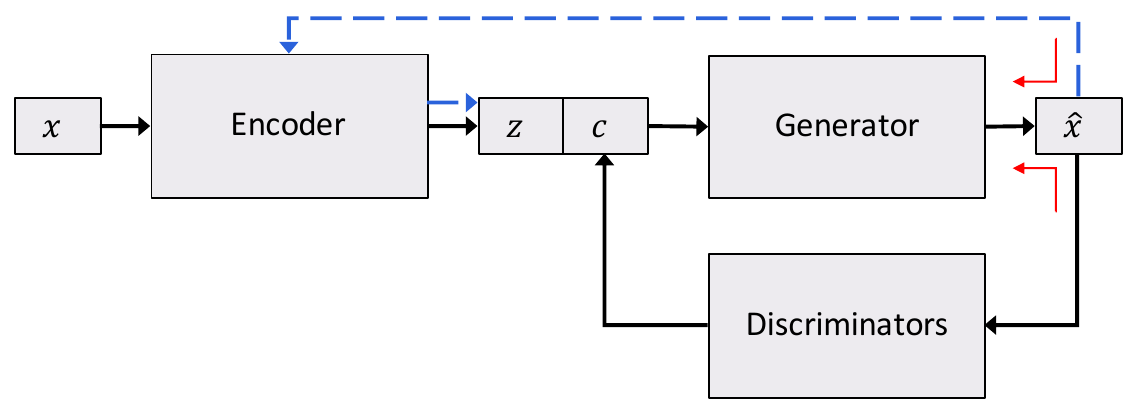
\includegraphics[width=0.5\textwidth]{images/toward1.png}
    \caption
    [نمایی نحوه آموزش مدل \towardctg.]
    {
        نمایی نحوه آموزش مدل \towardctg. خط‌های آبی و سفید جهت حرکت داده و خط‌های قرمز جهت انتفال گرادیان را مشخص می‌کنند \cite{toward}.}
    \label{fig:toward}
\end{figure}
همان‌طور که در شکل \ref{fig:toward} مشخص است، این مدل از ۳ بخش کلی تشکیل شده است؛ یک کدگذار، یک مولد و یک یا چند \discriminator{} که در شکل به جهت سادگی تنها یک نمونه از آن آورده شده است. اگر $c$ نشانگر شرط مورد نظر باشد، وظیفه کدگذار کد کردن جمله ورودی به فضای نهانی است که $c$ در آن ظاهر نشده باشد؛ از سوی دیگر مولد یا در ادبیات مدل‌های پیشین همان کدگشا وظیفه برگرداندن متغیر نهان بدست آمده از کدگذار به جمله اصلی البته با در نظر گرفتن شرط $c$ را داشته و در نهایت \discriminator{} موظف به نظارت بر وجود و رعایت شرط $c$ در جمله تولید شده توسط مولد است. در واقع می‌توان مدل را به صورت یک \vae{} شرطی به همراه یک شبکه \discriminator{} دید که وظیفه نظارت بر شرط مورد نظر را دارد. جهت آموزش این مدل و در نظر گرفتن ویژگی‌های ذکر شده، تابع هزینه از چندین قسمت تشکیل شده است که به اختصار راجع به آن‌ها توضیح داده خواهد شد.
\paragraph*{آموزش کدگذار و مولد}
مطابق با آنچه توضیح داده شد اولین بخش از تابع هزینه مربوط به تابع هزینه شبکه‌های \vae{} شرطی ساده بوده که کنترل‌کننده وظیفه کد کردن و برگرداندن آن به جمله با ویژگی مورد نظر را بر عهده دارد. اگر $E$ کدگذار، $G$ مولد و $D$ \discriminator{} باشد، خواهیم داشت:
\begin{equation}
\begin{split}
L_{VAE} (E, G) =& \expected_{\bff{x} \sim p_{data}} [KL (q_E(\bff{Z}|\bff{x}) || N(\textbf{\latin{0}},\textbf{\latin{I}})) - \expected_{\bff{z} \sim q_E(\bff{Z}|\bff{x}), c \sim q_D(C|\bff{x})} [\log p_G(\bff{x}|\bff{z},c)]].
\end{split}
\end{equation}
از سوی دیگر باید جمله تولیدی توسط مولد حامل ویژگی مورد نظر باشد \cite{toward}. بنابراین تابع هزینه ذیل در نظر گرفته شده است:
\begin{equation}
\begin{split}
L_{att, c} (G) =& -\expected_{\bff{z} \sim p(\bff{Z}), c \sim p(C)} [\log q_D(c|G(\bff{z}, c))]
\end{split}
\end{equation}
که $p(c)$ و $p(\bff{z})$
\trans{توزیع پیشین}{Prior distribution}
تعریف شده روی متغیرهای مربوطه هستند. به عبارت دیگر ابتدا تعدادی نمونه $z$ و $c$ با استفاده از توزیع‌های پیشین تعریف شده ایجاد نموده و سپس مولد بایستی جملاتی را تولید نماید که درست‌نمایی شروط در \discriminator{}‌های مربوطه بیشینه شود.\\
آخرین تابع هزینه‌ای که برای این بخش از مدل در نظر گرفته شده مربوط به حذف وابستگی بین متغیرهای $z$ و $c$ است. به عبارت دیگر مولد بایستی $z$ و $c$ را به جمله‌ای تبدیل نماید که اگر این جمله توسط کدگذار مجددا کد گردد، همان $z$ اولیه بدست آید و جنبه دیگری غیر شروط مورد نظر در جمله تغییر نکرده باشد \cite{toward}. این تابع به شکل زیر تعریف گردیده است:
\begin{equation}
\begin{split}
L_{att, z} (G) =& -\expected_{\bff{z} \sim p(\bff{Z}), c \sim p(C)} [\log q_E(\bff{z}|G(\bff{z}, c))].
\end{split}
\end{equation}
در واقع از سوی دیگر می‌توان کدگذار را به عنوان یک \discriminator{}‌ مشاهده کرد که وظیفه نظارت بر حفظ محتوای جمله غیر از شروط مورد نظر را دارد.
\paragraph*{آموزش دسته‌بند}
بخش دیگر مربوط به آموزش دسته‌بند می‌باشد؛ اینکه دسته‌بند برچسب شرط هر جمله را به درستی پیش‌بینی کند. لازم به ذکر است که برای هر ویژگی یا شرط، یک دسته‌بند مستقل وجود دارد. برای مثال اگر یک ویژگی زمان فعل و دیگری قطبیت آن باشد، دو دسته‌بند، یکی برای زمان فعل و دیگری برای قطبیت آموزش داده خواهد شد \cite{toward}. بخش اول تابع هزینه شبکه دسته‌بند به شکل ذیل است:
\begin{equation}
\begin{split}
L_{s} (D) =& -\expected_{(\bff{x},c) \sim p_{data}} [\log q_D(c|\bff{x})].
\end{split}
\end{equation}
علاوه بر تابع هزینه فوق، حالتی دیگری نیز که بر اساس نمونه‌برداری از فضای نهان شکل می‌گیرد، وجود دارد و به صورت زیر نوشته می‌شود:
\begin{equation}
\begin{split}
L_{u} (D) =& -\expected_{\bff{z} \sim p_\bff{Z}(\bff{Z}), c \sim p(C), \bff{x} \sim p_G(\bff{X}|\bff{z},c)} [\log q_D(c|\bff{x}) + \beta H(q_D(C'|\bff{x}))]
\end{split}
\end{equation}
که $H(q)$ آنتروپی توزیع $q$ و $\beta$ ضریب تنظیم کننده است که بیشنیه میگردد \cite{toward}؛ علت این موضوع نیز آن است که به دلیل امکان وجود خطا در خروجی \decoder{}، \classifier{} نمیبایستی با قطعیت راجع به برچسب آن اظهار نظر کند؛ در واقع این تابع هزینه به نوعی وظیفه \augmentation{} دارد.
در نهایت توابع هزینه به شکل زیر خواهند بود:
\begin{equation}
\begin{split}
L (D) &= L_{s} (D) + \lambda_u L_{u} (D)\\
L (G) &= L_{VAE} (G) + \lambda_c L_{att, c} (G) + \lambda_z L_{att, z} (G)\\
L (E) &= L_{VAE} (E)
\end{split}
\end{equation}
که $(\lambda_s, \lambda_u, \lambda_c , \lambda_z)$ همگی ضرایب تنظیم‌کننده هستند. از دیگر نقاط قوت این مدل باید به دو مورد زیر نیز اشاره نمود:
\renewcommand{\labelitemi}{$\bullet$}
\begin{itemize}
    \item
    
    آموزش
    \trans{نیمه‌نظارتی}{Semi-supervised}:
    همان‌طور که در روابط و نمای کلی مدل مشخص است، تابع هزینه $L_{VAE}$ نیازی به داده برچسب زده شده نداشته و به شکل \semisupervised{} آموزش می‌بیند. در واقع برای آموزش کل مدل به تعداد زیادی جمله بدون برچسب و تعداد کمتری که در حدود ۳۰۰ جمله که در مقاله ادعا شده است برای برچسب‌زنی نیاز است.
    \item
    عدم نیاز به داده 
    \trans{جفت برچسب زده شده}{Jointly labeled}:
    از آنجا که هر شرط مستقل از سایر شروط و برای هر یک، یک دسته‌بند و آموزش مجزا در نظر گرفته شده است، بنابراین نیازی به داده جفت برچسب‌زده شده نیست.
\end{itemize}

\subsection{مدل‌های مبتنی بر \gan{}}
\subsubsection{\cgan{}}
در مورد\gan{} نیز شرایطی مشابه \cvae{} حاکم است و شرط به مولد و \discriminator{}، ورودی داده می‌شود \cite{cgan} و رابطه آن به شرح زیر است:
\begin{align}
	\mcal{V}_\text{CGAN}(D, G) =
	\expected_{(\bff{x}, c) \sim \prob_\text{Data}} [\log D(\bff{x}|c)] +
	\expected_{c \sim p(C), \bff{z} \sim N(\bff{0}, \bff{I}),\bff{x} \sim p_G(\bff{X}|z,c)} [\log 1 - D(\bff{x}|c)]
\end{align}
که نسبت به $D$ بیشینه و نسبت به $G$ کمینه می‌گردد.
\begin{figure}[H]
	\centering
	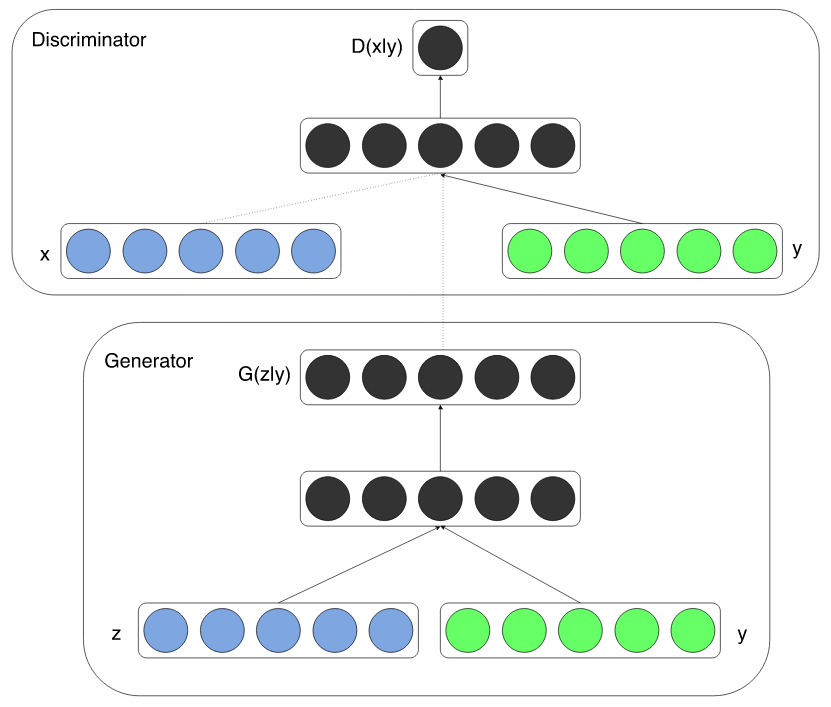
\includegraphics[width=.7\textwidth]{images/cgan.png}
	\caption{نمایی از \cgan{} \cite{cgan}}
    \label{fig:chap2:cgan}
\end{figure}
لازم به ذکر است که مجددا در رابطه فوق مشکل گذر گرادیان وجود دارد و معمولا از روش‌هایی مانند آنچه در بخش \ref{chap2:seqgan} (بر پایه یادگیری تقویتی) است، استفاده می‌شود. نمایی از \cgan{} در شکل \ref{fig:chap2:cgan} آمده است.

\subsubsection{
    تولید جملاتِ با تمایل، با استفاده از شبکه‌های تخاصمی مخلوط
     (\lr{SentiGAN})\protect\LTRfootnote{Generating Sentimental Texts via Mixture Adversarial Networks (SentiGAN)}
}
در این مدل به منظور تولید جمله با $C$ قطبیت معین، به ازای هر مقدار شرط یک مدل مولد مجزا و یک
\trans{دسته‌بند}{Classifier} $C+1$
کلاسه آموزش می‌دهد \cite{sentigan}؛ در این دسته‌بند یک دسته نشانگر داده مصنوعی و سایر دسته‌ها نشان‌گر مقادیر مختلف شرط هستند. در واقع هر مولد سعی در تولید جمله‌ای دارد که از نظر \classifier{} جمله از دسته شرط مرتبط تشخیص داده شده و در مقابل \classifier{} سعی بر نسبت دادن تمام جملات تولید شده توسط مولد‌ها را به دسته $C+1$ام و جملات دادگان اصلی به دسته متناظرشان را دارد و از این جهت همچنان یک \minmaxgame{} در جریان است. اگر
$\{ \bff{x}^n \}_{n=1}^N$
نمونه‌های از توزیع مولد $c$ام با حداکثر طول $T$ باشد، تابع هزینه مدل مولد $c$ام به شرح زیر است:
\begin{align}
	\mcal{L}_\text{SentiGAN}(G_c) = \frac{1}{N}
	\sum_{\bff{x}^n} \sum_{t=1}^{T}
	G_c(\bff{x}^n_t|\bff{x}^n_{1:t-1})
	V_{D_c}(\bff{x}^n_{1:t}, G_c)
\end{align}
که $D_c$ امتیاز \discriminator{} برای دسته $c$ام و تابع $V_{D_c}(., G_c)$ نیز پاداش نسبت داده شده به حرکت $t$ام از مولد $c$ است که برای محاسبه آن مجددا مانند مدل \lr{SeqGAN} (بخش \ref{chap2:seqgan}) از  \montecarlosearch{} برای تخمین پاداش این حرکت استفاده می‌شود. تعریف صوری این پاداش به صورت زیر است:
\begin{align}
	V_{D_c}(\bff{x}_{1:t}, G_c) = \frac{1}{N'} \sum_{n'=1}^{N'} (1 - D_c(\bff{x}_{1:t}, \bff{x}^{n'}_{t+1:T}))
\end{align}
در واقع با ثابت نگه‌داشتن $\bff{x}_{1:t}$،
$N'$
بار جمله را با $G_c$ تکمیل کرده و در نهایت امتیاز \discriminator{} به  $N'$ جمله میانگین گرفته می‌شود. واضح است که برای حرکت آخر (زمانی که $t=T$ است) چنین فرآیندی انجام نمی‌گیرد و از امتیاز \discriminator{} به کل جمله استفاده می‌شود \cite{sentigan}. قابل توجه است که $\mcal{L}_\text{SentiGAN}(G_c)$ با تابع هزینه \wgan{} نیز شبیه بوده، گرچه شرط \lr{K-Lipschitz} بودن برای آن رعایت نشده است
( $G_c(.)V_{D_c}(.)$
به عنوان تابع \critic{} در نظر گرفته شده است).
\\
تابع هزینه دسته‌بند نیز به صورت زیر تعریف می‌شود \cite{sentigan}:
\begin{align}
	\mcal{L}_\text{SentiGAN} (D) =
	- \sum_c \expected_{\bff{x} \sim p_{G_c}} \log D_{C+1} (\bff{x})
	- \expected_{\bff{x} \sim p_\text{Data}(.|c)} \log D_c(\bff{x})
\end{align}

مشخص است که با افزایش تعداد شرط‌ها، این مدل مقیاس‌پذیر نخواهد بود. برای مثلا اگر بخواهیم دو شرط ۳ و ۴ مقداره را مدل کنیم به ۱۲ مدل مولد نیاز است.
\subsubsection{
    مدل مولد برای تولید متن با شرط‌های مقدار گسسته
(\lr{CSGAN})\protect\LTRfootnote{A Generative Model for Category Text Generation (CSGAN)}}
این مدل نیز شباهت زیادی به مدل \cgan{} دارد. نکته اصلی تفاوت آن با \cgan{} در داشتن سیگنال پاداشی متفاوت است. در \cgan{}،
\discriminator{}
ضمن دریافت جفت جمله و شرط، احتمال نسبت به دسته واقعی یا مصنوعی بودن آن را تعیین می‌کرد؛ از این احتمال به عنوان پاداش در ساختار \reinforce{} برای حل گذر گرادیان استفاده شد. در این مقاله علاوه بر \discriminator{} ذکر شده، یک \classifier{} نیز به کار گرفته شده است و از ترکیب امتیاز واقعی بودن و تعلق جمله به دسته شرط مورد نظر، سیگنال پاداشی غنی‌تری ساخته شده است \cite{csgan}. ضمن حفظ ساختار کلی \cgan{}، دسته‌بند $D_C$ با تابع هزینه ذیل آموزش داده می‌شود:
\begin{align}
	\mcal{L}_\text{CGAN} (D_C) =
	-\expected_{(\bff{x}, c) \sim p_\text{Data}} [\log D_C(c|\bff{x})]
	-\expected_{c \sim p_C, \bff{x} \sim \prob_G(.|c)} [\log D_C(c|\bff{x})]
\end{align}
اگر \discriminator{} را با $D_R$ نشان دهیم، تابع پاداش نیز به شکل زیر تغییر می‌کند:
\begin{align}
	\text{Reward} (\bff{x}, c) =
	\frac{2 D_R(\bff{x},c)D_C(c|\bff{x})}
	{D_R(\bff{x},c) + D_C(c|\bff{x})}
\end{align}
در واقع چه طبیعی نبودن جمله و چه عدم تعلق جمله مورد نظر به دسته شرط مورد نظر باعث جریمه مولد خواهد شد و بالعکس.

\section{برخی مفاهیم دیگر}
در این بخش دو مطلب دیگر که یکی رویکرد آموزشی نوین و دیگری معماری نوینی که در حوزه متن اخیرا مورد توجه قرار گرفته است، توضیح داده خواهد شد.
\subsection{\normalizingflownets{}} \label{chap2:flow}
در کنار دو عضو بزرگ از خانواده شبکه‌های مولد مبتنی بر \vae{} و \gan{}، نوع دیگری از شبکه‌ها به نام 
\trans{شبکه‌های مبتنی بر جریان نرمال‌کننده}{Normalizing Flow Networks}
وجود دارند. یکی از مشکلات اساسی ما در این دو نوع \vae{} و \gan{} این است که توانایی محاسبه \likelihood{} به صورت کارا و بدون استفاده از کران‌های پایین و یا بالا وجود ندارد. برای مثال در \vae{} کران پایین \likelihood{} را بیشینه کرده \cite{vae} و در \gan{}‌ها نیز از تابع هزینه دیگری استفاده می‌شود و در مورد رابطه آن با \likelihood{} صحبت شفافی نمی‌توان کرد \cite{gan} (عدم امکان محاسبه \likelihood{} در \gan{} به صورت کلی بیان شد؛ این در حالی است که در حوزه متن امکان محاسبه آن وجود دارد).  بر خلاف این دو دسته، خانواده \normalizingflownets{} توانایی نمونه‌گیری و محاسبه \likelihood{} به صورت کارا را داشته و یا حداقل سعی بر این موضوع دارند \cite{flow_survey}. بنابراین امکان بهینه‌سازی مدل نسبت به تابع هزینه‌ای بر مبنای مقدار دقیق \likelihood{} امکان پذیر است. از سوی دیگر همان طور که تا به اینجا توضیح داده شد، سختی‌ها و نقاط ضعفی از قبیل تنوع نداشتن نمونه‌ها در \gan{} و یا صفر شدن بخش \lr{KL} در \vae{} وجود دارد. این در حالیست که در \normalizingflownets{} با بهینه‌سازی بر اساس \likelihood{} مشکل کم بودن تنوع نمونه‌ها وجود نداشته و یا مشکلات آموزش مانند آنچه ذکر شد، گزارش نشده است. البته این نکته قابل ذکر است که در صورت کم بودن ظرفیت مدل نسبت به توزیع هدف مورد نظر، تابع هزینه مبتنی بر \likelihood{} رفتار \meanseeking{} از خود بروز داده و توزیعی را یاد خواهد گرفت که تمام نقاط را پوشش دهد. بدیهیست که ممکن است برای پوشش دادن تمام نقاط نقاطی نامطلوب را نیز پوشش دهد.
\subsubsection{مفاهیم پایه}
فرض کنید
${\bf{ Z}} \in \mathbb{R}^{D}$
متغیر تصادفی با تابع چگالی احتمال مشخص
$p_{\bf Z}: \mathbb{R}^D$
و $\bf f$ تابعی معکوس پذیر و
${\bf Y} = {\bf f}({\bf Z})$
است. حال با استفاده از قانون تغییر متغیر می‌توان رابطه زیر را نوشت:
\begin{align}  \label{eq:flow_target_dist}
p_{\bf Y}({\bf y}) = & p_{\bf Z}({\bf g}({\bf y}))
|\text{det} ~ \text{D} {\bf g}({\bf y})|
\nonumber                                          \\
=                    & p_{\bf Z}({\bf g}({\bf y}))
|\text{det} ~ \text{D} {\bf f}({\bf g}({\bf y}))|^{-1}
\end{align}
که $\bf g$ تابع معکوس $\bf f$ و
$\text{D} {\bf g}({\bf y}) = \frac{\partial {\bf g}}{\partial {\bf y}}$
ماتریس ژاکوبین تابع $\bf g$ و
$\text{D} {\bf f}({\bf z}) = \frac{\partial {\bf f}}{\partial {\bf z}}$
ماتریس ژاکوبین تابع $\bf f$ است. تابع چگالی احتمال حاصل از اعمال تابع $\bf f$ به توزیع پایه را با
$f_*p_{\bf Z}$
نشان خواهیم داد.

در ادبیات مدل‌های مولد، تابع $\bf f$ به عنوان مولد، توزیع پایه
$p_{\bf z}$
را به توزیعی پیچیده‌تر تبدیل می‌کند که به حرکت از توزیع پایه به توزیع نهایی را جهت مولد می‌نامند. به منظور نمونه‌برداری از توزیع نهایی نیز می‌توان از توزیع پایه نمونه برداری کرده و با استفاده از تابع
${\bf y} = {\bf f} ( {\bf z} )$
به نمونه از توزیع نهایی رسید. در جهت مخالف، برای تبدیل توزیع نهایی به توزیع پایه که معمولا توزیع گاوسی نرمال انتخاب می‌شود، از تابع $\bf g$ بهره برده می‌شود. به همین دلیل انتخاب نام جریان نرمال‌کننده بدون هدف نبوده و در واقع جهت مخالف مربوط به تبدیل توزیع پیچیده نهایی به توزیع پایه گاوسی نرمال است \cite{flow_survey}.
\\
به طور کلی اگر تابع $\bf f$ یک تبدیل پیچیده باشد، توانایی تولید هر توزیعی وجود خواهد داشت؛ به عبارت دیگر به ازای هر توزیع هدف
$ p_{\bf Y}({\bf y})$
تابع $\bf f$ای وجود خواهد داشت که
$ p_{\bf Y}({\bf y}) = f_*p_{\bf Z}$.
اما به منظور آموزش و نمونه‌گیری کارا، نیاز است تا این توابع ویژگی‌های خاصی به شرح ذیل داشته باشند \cite{flow_survey}:
\begin{itemize}
    \item
    معکوس‌پذیر باشند. ممکن است تابع معکوس در جهت نمونه‌گیری و یا جهت نرمال‌ساز به کار برده شود.
    \item
    به اندازه کافی پیچیده باشند تا بتواند توزیع داده اصلی را مدل کنند.
    \item
    به لحاظ محاسباتی کارا باشند. برای محاسبه \likelihood{} یک نمونه و نمونه‌گیری نیاز است تا هر دو جهت نمونه‌گیری و نرمال‌ساز به صورت کارا محاسبه شوند. علاوه بر این، طبق رابطه \ref{eq:flow_target_dist} برای محاسبه  \likelihood{} یک نمونه در توزیع نهایی، به محاسبه کارای دترمینان ماتریس ژاکوبین تابع $\bf f$ نیاز است. بنابراین بایستی دترمینان ماتریس ژاکوبین تابع $\bf f$ نیز به صورت کارا محاسبه شود.
\end{itemize}
این خانواده از مدل‌های مولد شامل چندین دسته هستند که در ادامه معرفی خواهند شد.
\subsubsection{جریان‌های
    \trans{درایه‌گرا}{Elementwise}}
یک فرم پایه از توابع غیرخطی معکوس‌پذیر را می‌توان از توابع \elementwise{} ساخت. فرض کنید تابع
$h: \mathbb{R} \rightarrow \mathbb{R}$
باشد و معکوس‌پذیر است. اگر
${\bf x} = (x_1, x_2, ..., x_D)^T$
خواهیم داشت:
\begin{gather}
{\bf f}({\bf x}) = (h(x_1), h(x_2), ..., h(x_D))^T
\end{gather}
برای محاسبه تابع معکوس به تابع $h^{-1}$ نیاز است و از آنجا که ماتریس ژاکوبین آن قطری است پس دترمینان آن ضرب المان‌های روی قطر آن خواهد شد. در واقع چنین تابعی مانند توابع فعال‌سازی مورد استفاده در شبکه‌های عصبی هستند؛ با این تفاوت که این توابع معکوس پذیر نیستند. برای مثال تابع \lr{ReLU} معکوس پذیر نیست اما \lr{ELU} است. به دلیل اینکه این توابع به صورت \elementwise{} عمل می‌کنند، پیچیدگی لازم را ندارند. مدل‌های بعدی سعی در پوشش این ضعف دارند \cite{flow_survey, realnvp, iaf, maf}.
\subsubsection{جریان‌های خطی}
یک تبدیل خطی به طور کلی به شکل زیر تعریف می‌شود:
\begin{align}
{\bf f}({\bf x}) = {\bf A}{\bf x} + {\bf b}
\end{align}
که $A \in \mathbb{R}^{D \times D}$ و $b \in \mathbb{R}^D$ پارامتر‌های این تبدیل هستند. دترمینان این تبدیل برابر با دترمینان ماتریس ${\bf A}$ بوده و برای معکوس آن نیاز به ${\bf A}^{-1}$ است.
این دو عملیات در حالت کلی با مرتبه زمانی
$O(D^3)$
قابل انجام هستند. اگر توزیع پایه از نوع توزیع‌های نمایی باشد، بعد از اعمال تبدیل فوق در خانواده توزیع‌های نمایی باقی می‌ماند. با این وجود، این دسته یکی از پایه‌های اصلی توابع پیچیده هستند. برای تقلیل زمان محاسبه دترمینان و معکوس تابع، به عناوین مختلف سعی در محدود کردن شکل آن‌ها شده تا این اعمال به صورت کارا انجام پذیرند. برای مثال از پارمتری کردن ${\bf A}$ به صورت پایین مثلثی یا بالا مثلثی بهره برده می‌شود تا دترمینان به صورت بسیار ساده و با ضرب المان‌های روی قطر بدست آید و ماتریس معکوس نیز در $O(D^2)$ محاسبه شود. از آنجا که قدرت این تبدیل وابسته به ترتیب اعمال شده به ابعاد است (هر بعد تابعی از بُعدهای قبل از خود است)، راهکارهای متفاوتی از قبیل تغییر ترتیب به صورت تصادفی و یا یافتن یک ماتریس تبدیل متعامد (حالت کلی‌تر تغییر ترتیب در بعدها) ارائه شده است \cite{flow_survey, glow}.
\subsubsection{جریان‌های
    \trans{اتصالی}{Coupling}
}
در این گونه از تبدیل‌ها، فضای ورودی به دو زیرفضا تقسیم می‌شود. اگر فضای ورودی را با
$\bff{x} \in \bb{R}^D$
نشان دهیم، دو زیرفضا از آن به صورت
$(\bff{x}^A, \bff{x}^B) \in \bb{R}^d \times \bb{R}^{D - d}$
، تابع معکوس‌پذیر
$\hat{\bff{f}}(.; \theta) : \bb{R}^D \rightarrow \bb{R}^D$
را در نظر بگیرید. یک جریان \coupling{}
$f : \bb{R}^D \rightarrow \bb{R}^D$
را به شکل زیر می‌توان تعریف نمود:
\begin{align}
\bff{y}^A = & \hat{\bff{f}} (\bff{x}^A; \Theta(\bff{x}^B))
\nonumber
\\
\bff{y}^B = & \bff{x}^B
\end{align}
که $\Theta(\bff{x}^B)$ یک تابع کاملا پیچیده از $\bff{x}^B$ است که به آن
\trans{شرطی‌کننده}{Conditioner}
، به تابع $\hat{\bff{f}}$ یک لایه \coupling{} و به کل تابع $\bff{f}$ یک جریان \coupling{} گفته می‌شود. نمایی از این جریان در شکل \ref{fig:chap2:flow_coupling} آمده است. معکوس‌پذیری این جریان در گرو معکوس‌پذیری لایه \coupling{} است و در این صورت به شکل زیر محاسبه می‌گردد:
\begin{align}
\bff{x}^A = & \hat{\bff{f}}^{-1} (\bff{y}^A; \Theta(\bff{y}^B))
\nonumber
\\
\bff{x}^B = & \bff{y}^B
\end{align}
ماتریس ژاکوبین این تابع نیز به صورت یک
\trans{ماتریس مثلثی بلوکی}{Block triangular matrix}
است که یکی از بلوک‌های آن ماتریس همانی و دیگری $\text{D}\hat{\bff{f}}$ است. بنابراین دترمینان  تابع $\bff{f}$ دترمینان برابر تابع $\hat{\bff{f}}$ است \cite{flow_survey, realnvp, glow}.

\begin{figure}[H]
    \centering
    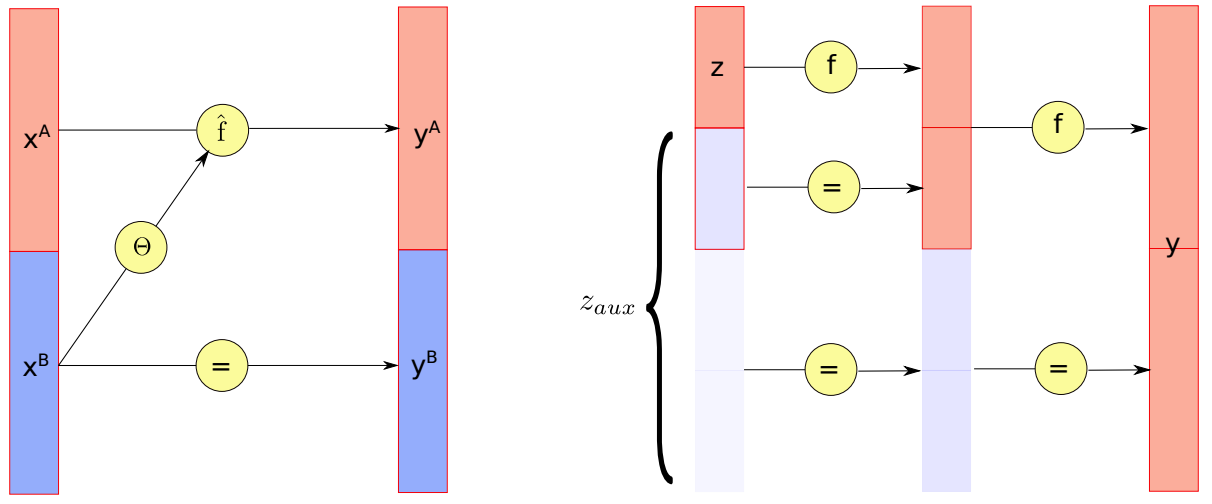
\includegraphics[width=.7\textwidth]{images/flow-survey1.png}
    \caption{
        نمایی از جریان‌های \coupling{}
        \cite{flow_survey}	}
    \label{fig:chap2:flow_coupling}
\end{figure}

در واقع قدرت اصلی این تابع در میزان پیچیده بودن تابع $\Theta$ است و می‌توان آن را با شبکه عصبی مدل نمود. لازم به ذکر است که این تابع می‌تواند تابعی از $\bff{x}^B$ نباشد و به عنوان اضافه کردن بُعد به کار بسته شود. اما مشکل این تبدیل در نحوه شکستن فضای ورودی به دو فضا است. روش‌های مختلفی نیز از جمله تغییر ترتیب ابعاد به صورت تصادفی برای حل این مشکل ارائه شده است.
\subsubsection{جریان‌های \autoregressive{}}
می‌توان مدل‌های \autoregressive{} را مدل‌هایی از جنس \normalizingflownets{} و نسخه غیر خطی ضرب ماتریس مثلثی در نظر گرفت \cite{flow_survey, iaf, maf}.
\\
مجددا اگر فضای ورودی با
$(x_1, x_2, ..., x_D) = \bff{x} \in \bb{R}^D$
نشان داده شود و
$\hat{\bff{f}} : \bb{R} \rightarrow \bb{R}$
یک تابع معکوس‌پذیر باشد، با داشتن یک ترتیب ثابت بر روی فضای ورودی، تابع \autoregressive{}
$\bff{y} = \bff{f} : \bb{R}^D \rightarrow \bb{R}^D$
به صورت زیر تعریف می‌شود:
\begin{align}
y_t = \hat{\bff{f}}(x_t; \Theta_t(x_{1:t-1}))
\end{align}
که $t= 2, 3, ..., D$
، $\Theta_t$
یک تابع پیچیده از $\bb{R}^{t-1}$ به فضای پارامترهای تابع $\bff{f}$ و $\Theta_1$ یک تابع ثابت است. در اینجا نیز به $\Theta_t$ یک \conditioner{} گفته می‌شود.
\\
از آنجا که $y_t$ تنها تابعی از $x_{1:t-1}$ است، ماتریس ژاکوبین این تابع نیز مثلثی بوده و بنابراین دترمینان آن از ضرب عناصر قطر آن بدست می‌آید. با داشتن تابع معکوس $\hat{\bff{f}}$، معکوس تابع $\bff{f}$ قابل محاسبه است؛ اما از آنجا که ساختار \autoregressive{} بر روی ابعاد حاکم است، بنابراین  باید هر بعد به صورت ترتیبی از ابعاد قبل به دست آید و درنتیجه نمی‌توان از پتانسیل موازی‌سازی \gpu{} بهره برد. به منظور موازی‌سازی در جهت نمونه‌گیری، می‌توان از ساختار شبکه‌های \lr{MADE} بهره برد. این شبکه به این صورت است که هر بُعد از آن تنها تابعی از ابعاد قبل از خود است. نمایی از این شبکه در شکل \ref{fig:chap2:made} آمده است \cite{made}.
\begin{figure}[h]
    \centering
    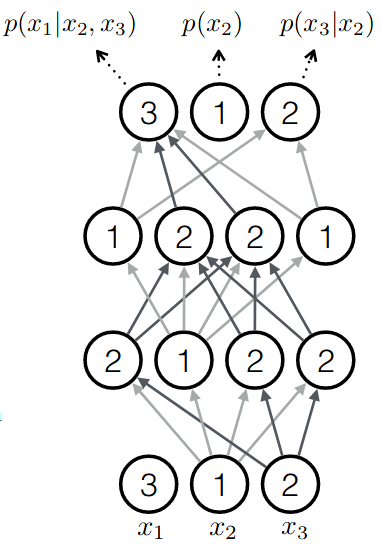
\includegraphics[width=.25\textwidth]{images/made.png}
    \caption{
        نمایی از مدل \lr{MADE}
        \cite{made}.
    }
    \label{fig:chap2:made}
\end{figure}
در صورت استفاده از ساختار شبکه \autoencoder{} نقابی برای تخمین توزیع (\lr{MADE})
\LTRfootnote{Masked Autoencoder for Distribution Estimation (MADE)}
در $\Theta$، به آن 
جریان \autoregressive{} نقابی (\lr{MAF})
\LTRfootnote{Masked Autoregressive Flow (MAF)}
گفته می‌شود \cite{maf}.

\begin{figure}[h]
    \centering
    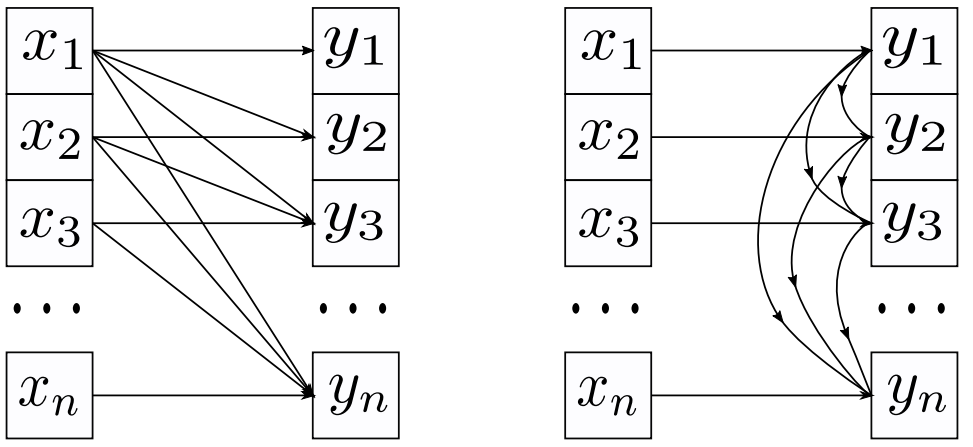
\includegraphics[width=.5\textwidth]{images/flow-survey2.png}
    \caption{
        تفاوت مدل‌های \lr{MAF} و \lr{IAF} به زبان تصویر \cite{iaf, maf, flow_survey}
    }
    \label{fig:chap2:mafvsiaf}
\end{figure}

مدل‌سازی تابع \autoregressive{}
$\bff{f}$
را می‌توان به صورت زیر نیز تعریف کرد:
\begin{align}
y_t = \hat{\bff{f}}(x_t; \Theta_t(y_{1:t-1}))
\end{align}
که در واقع عکس روش \lr{MAF} است. به همین دلیل این روش را جریان \autoregressive{} معکوس (\lr{IAF})
\LTRfootnote{Inverse Autoregressive Flow (IAF)}
می‌نامند \cite{iaf, flow_survey}. در واقع در \lr{MAF} رفتن از توزیع پایه به توزیع نهایی کُند و رفتن از توزیع نهایی به توزیع پایه سریع است؛ در حالی که \lr{IAF} نمونه‌برداری سریع اما جریان نرمال‌کننده کندی دارد و بایستی بسته به نیاز از آن‌ها بهره برد. تفاوت این مدل در شکل \ref{fig:chap2:mafvsiaf} مشخص است.
نکته قابل ذکر در مورد دسته \autoregressive{}  از \normalizingflownets{} این است که در  بعضی موارد اثبات شده است که این خانواده از توابع، توانایی مدل کردن هر تابعی را داشته و به اصطلاح یک
\trans{تخمین‌‌گر عمومی}{Universal approximator}
هستند \cite{flow_survey}.
\subsubsection{لایه‌های \coupling{}}
تا به اینجا در مورد خانواده‌های مختلف \normalizingflownets{} صحبت شد. در تمام آن‌ها از توابع معکوس‌پذیر استفاده شده اما در مورد ساختار آن‌ها توضیحی داده نشد. در این بخش به توضیح تعدادی از توابع معکوس پذیر مورد استفاده پرداخته خواهد شد.
\paragraph*{لایه
    \coupling{} \trans{هم‌نسبی}{Affine}}
این لایه‌های خطی، ساده‌ترین و رایج‌ترین لایه‌های مورد استفاده در \normalizingflownets{} هستند. اگر لایه مورد نظر با $\hat{\bff{f}}: \bb{R} \rightarrow \bb{R}$ نشان داده شود، به صورت زیر تعریف می‌شود:
\begin{align}
\hat{\bff{f}} (x; \theta) = \theta_1 x + \theta_2, \theta_1 \neq 0, \theta_2 \in \bb{R}
\end{align}
این لایه در مدل‌های بسیاری از جمله \cite{iaf, maf} استفاده شده است.
\paragraph*{لایه \coupling{}
    غیر خطی درجه دو}
نوع پیشرفته‌تر لایه ذکر شده، نسخه غیرخطی آن‌ها می‌باشد. به این صورت که تابع $\hat{\bff{f}}$ برای مثال به صورت یک تابع درجه ۲ در نظر گرفته می‌شود. به طور واضح چنین تابعی بایستی معکوس‌پذیر باشد؛‌ به همین دلیل از شروط مختلفی برای برآوردن آن استفاده می‌گردد. برای مثال این تابع می‌تواند به صورت زیر تعریف شود:
\begin{align}
\hat{\bff{f}}(x; \theta) = ax + b + \frac{c}{1 + (dx + h)^2}
\end{align}
تحت شرایطی پارامترهای $\theta=[a,b,c,d]$ یک تابع معکوس پذیر خواهند ساخت و به این هدف، نیاز به محاسبه ریشه تابع فوق که یک تابع درجه ۳ است، خواهد بود \cite{flow_survey}.
\paragraph*{لایه \coupling{} \spline{}}
این نام که شاید بیش‌تر در محاسبات عددی شنیده شود، به معنی یک تابع
\trans{تکه‌ای چند جمله‌ای}{Piece-wise polynomial}
است. در واقع اگر $K+1$ نقطه وجود داشته باشد، فواصل بین هر دو نقطه با یک تابع چندجمله‌ای مدل خواهد شد (در واقع $K$ تابع وجود خواهد داشت). حال این توابع باید از نقاط تعیین شده عبور کنند و همچنین در مجموع معکوس‌پذیر باشند. برای محاسبه تابع معکوس نیز پس از تعیین اینکه نقطه مورد نظر مربوط به کدامین تابع از $K$ تابع است، ریشه‌ی معادله مربوطه، جواب خواهد بود \cite{flow_survey}.
\paragraph*{لایه \coupling{} عصبی}
نوع کلی‌تری از این لایه‌ها نیز موجود است که با یک شبکه عصبی مدل می‌شوند. به مانند قبل،‌ باید این تابع معکوس‌پذیر باشد؛ برای مثال اگر وزن‌های این تابع همگی مثبت و توابع فعال‌سازی آن یکنوا باشند، این شبکه یک تابع معکوس‌پذیر خواهد بود. در رابطه با این مورد ادعای \univapprox{} نیز وجود دارد \cite{flow_survey}.
\\\\
علاوه بر دسته‌های ذکر شده، دسته‌های دیگری نیز وجود دارند که از حوصله این بحث خارج است. لازم به ذکر است که خانواده \normalizingflownets{} اخیرا بیشتر مورد توجه قرار گرفته و می‌تواند حوزه تحقیقی مورد توجهی باشد.
\subsection{معماری \transformer{}}
معماری‌های معمول استفاده شده در حوزه پردازش متن بیشتر شامل \lstm{} و \cnn{} هستند. اخیرا معماری دیگری به نام \transformer{} مورد توجه قرار گرفت که مخصوص پردازش داده‌های به صورت دنباله بوده و پایه بسیاری از مدل‌های \stateoftheart{} است. در ادامه به معرفی این معماری و اجزای آن پرداخته خواهد شد.
\\
این مدل معماری نیز در گروه مدل‌های
\trans{دنباله به دنباله}{Sequence to sequence}
جای گرفته و از \encoder{} و \decoder{} تشکیل شده است. اگر یک جمله با طول $n$ را با $\bff{x} = (x_1, ..., x_n)$  نشان داده شود، \encoder{} با گرفتن دنباله کلمات $\bff{x}$ (یا هر واحد مورد استفاده دیگر)، این دنباله  را به دنباله بردار‌های پیوسته $\bff{z} = (z_1, ..., z_n)$ تبدیل می‌کند. \decoder{} نیز با گرفتن $\bff{z}$ دنباله کلمات مقصد $\bff{y} = (y_1, ..., y_m)$ خروجی می‌دهد. با اینکه معماری \encoder{} به صورت \autoregressive{} نیست اما \decoder{}، واحدی برای کنترل و ایجاد حالت \autoregressive{} را در خود جای داده است \cite{transformer}.
\begin{figure}[H]
    \centering
    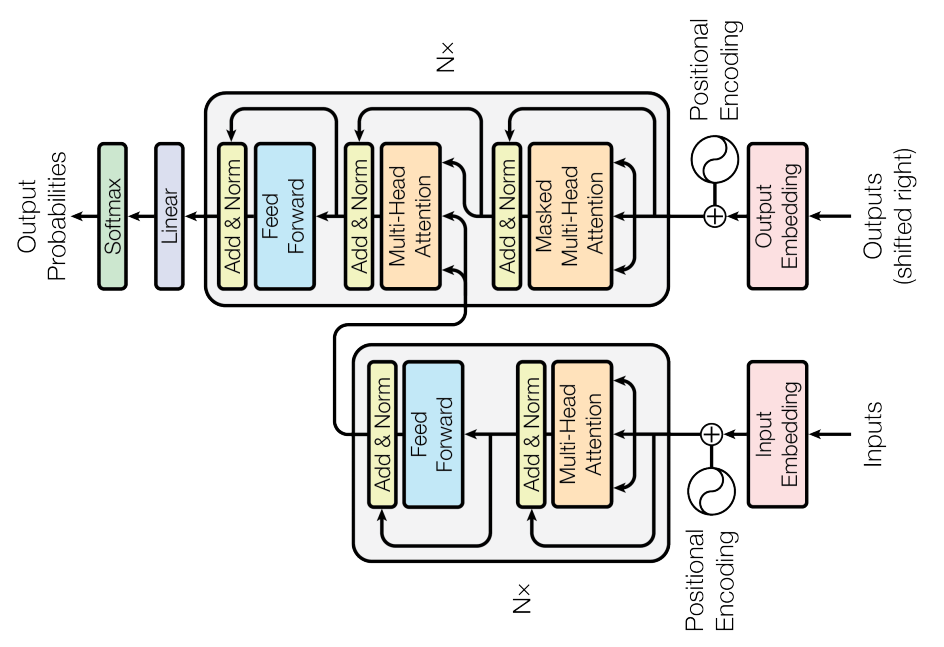
\includegraphics[width=.7\textwidth, angle=-90]{images/attention3.png}
    \caption{
        نمایی از معماری کلی \transformer{} \cite{transformer}}
\end{figure}

\paragraph*{\encoder{}}
\encoder{}
از پشته‌ای $N$ لایه یکسان تشکیل شده است. هر لایه شامل دو زیر لایه است. اولین زیر لایه مربوط به نوعی مکانیزم توجه به نام
\trans{خودتوجه چند سر}{Multi-head Self-attention}
و زیر لایه دوم یک لایه
\trans{تمام متصل}{Fully connected}
است. لازم به ذکر است که در هر زیرلایه از اتصالات
\trans{باقی‌مانده}{Residual}
و
\trans{نرمال‌کننده لایه}{Layer normalization}
استفاده شده است\cite{transformer}.
\paragraph*{\decoder{}}
\decoder{}
نیز از پشته کردن $N$ لایه تشکیل شده است. هر لایه علاوه بر واحد‌های ذکر شده برای \encoder{}، زیرلایه سومی نیز دارد که شامل
\trans{توجه چند سر}{Multi-head Attention}
به خروجی \encoder{} است. در \decoder{} نیز از اتصالات \residual{} و \layernormalization{} استفاده شده است. واحد \multiheadselfattention{} تفاوت کوچکی با واحد مشابه \encoder{} دارد تا در پیشبینی هر کلمه در خروجی، تنها تابعی از کلمات قبل از خود بوده و \autoregressive{} باشد \cite{transformer}.
\\
یک مکانیزم توجه را می‌توان نگاشتی از بردار
\trans{پرسمان}{Query}
و یک مجموعه \keyvaluepair{} به یک بردار در نظر گرفت که \query{}، کلیدها و مقدارها همگی بردارند. بردار خروجی از جمع وزن‌دار بردارهای مقدار و هر وزن نسبت داده شده به بردار مقدار، با تابعی از بردار \query{} و کلید بدست می‌آید. در ادامه به شرح دقیق‌تر این مکانیزم پرداخته خواهد شد.
\subsubsection{مکانیزم
    \trans{توجه با استفاده از ضرب داخلی مقیاس شده}{Scaled Dot-Product Attention}}
این مکانیزم توجه که نام \dotattention{} بر آن نهاده شده است بر روی بردارهای \query{} و کلید $d_k$ بعدی و بردارهای مقدار $d_v$ بعدی اعمال می‌شود. امتیاز هر بردار مقدار با استفاده از ضرب داخلی بردار \query{} در بردار کلید متناظر آن بدست آمده و در نهایت با اعمال تابع \softmax{} بر روی آن وزن مربوطه محاسبه می‌گردد. لازم به ذکر است که برای کنترل واریانس امتیاز هر بردار مقدار، امتیازات قبل از اعمال تابع \softmax{} تقسیم بر $\sqrt{d_k}$ می‌شوند \cite{transformer}.
\begin{figure}[H]
    \centering
    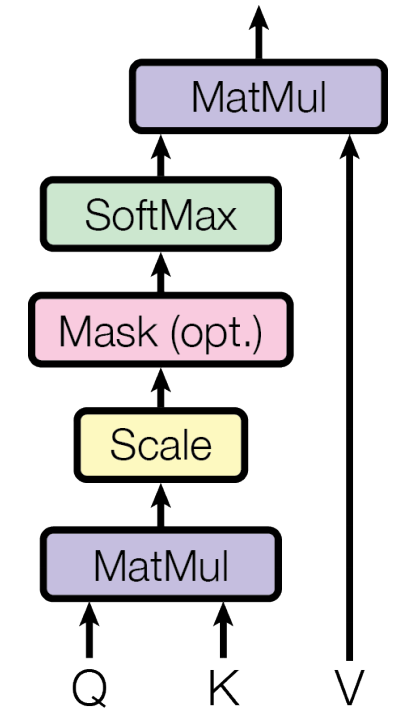
\includegraphics[width=.25
    \textwidth]{images/attention1.png}
    \caption{نمایی از \dotattention{}
        \cite{transformer}.}
\end{figure}
این مکانیزم به صورت زیر می‌توان تعریف کرد:
\begin{align}
\text{Attention}(Q, K, V) = \text{softmax}(\frac{QK^T}{\sqrt{d_k}})V
\end{align}
که
$Q \in \bb{R}^{n \times d_k}$،
$K \in \bb{R}^{n \times d_k}$ و
$V \in \bb{R}^{n \times d_v}$
به ترتیب بردارهای \query{}، کلید و مقدار هستند.
ویژگی \autoregressive{} در همین نقطه به مدل تزریق می‌شود. اگر امتیاز یک بردار مقدار $-\infty$ شود، وزن نسبت داده شده به این بردار پس از اعمال \softmax{} برابر با صفر خواهد بود؛ بنابراین می‌توان به طور دلخواه تاثیر هر بردار مقدار را با نسبت دادن  امتیاز $-\infty$ به آن، صفر کرد. به ماتریس $n \times n$ بُعدی که ردیف $i$ام آن بیان کننده مکان‌های قابل توجه برای کلمه $i$ام است، ماتریس
\trans{نقاب}{Mask}
گفته می‌شود (یک برای مکان‌های قابل توجه و $-\infty$ برای مکان‌های غیرقابل توجه) \cite{transformer}.

\subsubsection{مکانیزم \multiheadattention{}}
این امکان وجود دارد که به جای یک بار اعمال تابع توجه بر بردارهای $d_\text{model}$ بُعدی ($d_\text{model}$ اندازه بردار ورودی است)، بردارهای \query{}، کلید و مقدار را با $h$ تبدیل خطی به ترتیب به $h$ فضای مختلف با ابعاد $d_k$، $d_k$ و $d_v$ بُعدی برده و پس از اعمال تابع توجه، نتایجشان را به یکدیگر متصل کرد. لازم به ذکر است که این عملیات‌ها همگی به موازات یکدیگر  قابل انجامند و می‌توان از پتانسیل موازی‌سازی \gpu{} بهره گرفت. در واقع \multiheadattention{} این امکان را به مدل می‌دهد تا با بردن بردارها به فضاهای متفاوت، از چندین فضای مختلف به مکان‌ها و ویژگی‌های مختلف نگاه کرده و در نتیجه به مکان‌های متفاوتی به صورت همزمان توجه کند \cite{transformer}.
\begin{gather}
\text{MultiHead}(Q, K, V) = \text{Concat}(\text{head}_1, ..., \text{head}_h)W^O \nonumber
\\
: \text{head}_i = \text{Attention}(QW_i^Q, KW_i^K, VW_i^V)
\end{gather}
که
$W_i^Q \in \bb{R}^{d_\text{model} \times d_k},
W_i^K \in \bb{R}^{d_\text{model} \times d_k},
W_i^V \in \bb{R}^{d_\text{model} \times d_v},
W^O \in \bb{R}^{hd_v \times d_\text{model}}$
ماتریس‌های تبدیل خطی هستند. لازم به ذکر است که $h \times d_v = d_\text{model}$ است.
\begin{figure}[H]
    \centering
    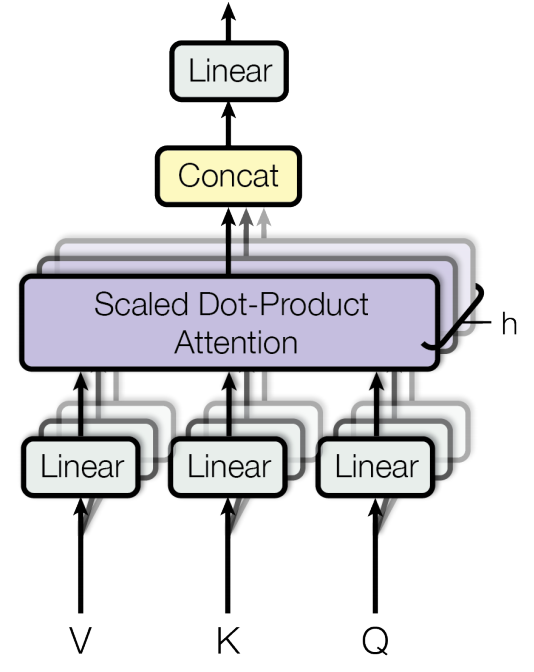
\includegraphics[width=.4
    \textwidth]{images/attention2.png}
    \caption{نمایی از \multiheadattention{}}
\end{figure}
تا به اینجا مکانیزم توجه در \transformer{} توضیح داده شد اما این مکانیزم به چه صورتی و در کجا استفاده شده است؟
\begin{itemize}
    \item
    در \decoder{} واحد \multiheadattention{} وجود دارد. در اینجا \query{} ها، خروجی لایه قبل \decoder{} و بردارهای مقدار و کلید خروجی‌های \encoder{} هستند. در واقع می‌توان از این مکانیزم تعبیر حافظه نیز داشت \cite{transformer}.
    \item
    در \encoder{} نیز از \multiheadselfattention{} نام برده شد. \multiheadselfattention{} همان \multiheadattention{} است اگر که بردار \query{}، کلید و مقدار آن یک چیز باشند. بنابراین به ازای هر کلمه، در هر لایه \encoder{}، به تمام خروجی‌های لایه قبل \multiheadselfattention{} زده می‌شود \cite{transformer}.
    \item
    مجددا در \decoder{} نیز از \multiheadselfattention{} استفاده شده است؛ با این تفاوت که در هر لایه، بردار متناظر با کلمه $i$ با استفاده از \mask{}‌های $-\infty$، تنها تابعی از بردار کلمات قبل‌تر از $i$ خواهد بود \cite{transformer}.
\end{itemize}

\subsubsection{بردار
    \trans{تعبیه مکانی}{Positional Embedding}}
از آنجا که ساختار معرفی شده، خاصیت \recurrence{} ندارد، در هیچ جایی اطلاعاتی راجع به فاصله کلمات نسبت به هم و موقعیتشان در جمله وارد مدل نمی‌شود؛ بنابراین نیاز است تا به نحوی موقعیت کلمات در بردار \embedding{} هر کلمه گنجانده شود که به آن \positionalembedding{} گفته می‌شود. بردار \positionalembedding{}
$PE$
که $d_\text{model}$ بُعدی است، به صورت زیر تعریف شده است \cite{transformer}:
\begin{align}
PE_{(pos, 2i)} = \sin ( pos / 10000^{2i/d_\text{model}}) \nonumber
\\
PE_{(pos, 2i+1)} = \cos ( pos / 10000^{2i/d_\text{model}})
\end{align}
که $pos$ شناسه مکانی مورد نظر است. در مورد نحوه انتخاب روش \encoding{} نیز این طور بیان شده است که
\positionalembedding{}  $i+k$
تابعی خطی از
\positionalembedding{} $i$
است بوده و قابلیت توسعه‌پذیری به جملات با طول‌های بیشتر که در حین آموزش دیده نشده است را ایجاد می‌کند \cite{transformer}. لازم به ذکر است که بردار \positionalembedding{} با بردار \embedding{} کلمه متناظرش جمع خواهد شد.
\newline
در این فصل سعی شد تا در ابتدا فاصله‌های معروف مورد استفاده و سپس مدل‌های زبانی غیر شرطی، به دلیل پایه‌ای بودن این \task{} نسبت به \task{} تولید شرطی، در دو دسته با فضای نهان و بدون فضای نهان، معرفی شوند. در این بین، مشکل عدم توجه به فضای نهان مطرح و راه‌حل‌هایی برای آن ارائه شد. در انتها نیز ضمن شرح معماری نوین \transformer{} و همچنین رویکردِ کمتر مورد توجه \normalizingflownets{}، رویکرد‌های متفاوت آموزش مدل‌های زبانی شرطی توضیح داده شده و مورد بررسی قرار گرفتند.
در فصل بعد ضمن مروری بر ضعف و قوت مدل‌های معرفی شده، مدل پیشنهادی جهت رفع مشکلات ذکر شده و همچنین توانایی در تولید متن به صورت شرطی ارائه خواهد شد.
